\subsection{Lịch sử và Động lực ra đời của mạng RNN}
Trong khi các mạng nơ-ron truyền thống (Feedforward Neural Networks) và CNN giả định rằng tất cả các đầu vào và đầu ra là độc lập với nhau, nhiều bài toán thực tế lại đòi hỏi khả năng xử lý dữ liệu có tính thứ tự (Sequential Data). Ví dụ, để hiểu một câu văn, bạn cần biết các từ đứng trước đó; hoặc để dự báo giá chứng khoán, bạn cần biết diễn biến giá trong quá khứ.

Mạng nơ-ron hồi quy (Recurrent Neural Network - RNN) được ra đời để giải quyết bài toán này. Lịch sử của RNN bắt đầu từ những năm 1980 với các mô hình như mạng \textit{Hopfield} và sau đó là mạng \textit{Elman} (1990) hay mạng \textit{Jordan}. Ý tưởng cốt lõi là tạo ra một vòng lặp trong kiến trúc mạng, cho phép thông tin được lưu giữ và truyền từ bước thời gian này sang bước thời gian khác.

\subsubsection{Các dạng kiến trúc RNN phổ biến}
Tùy thuộc vào đầu vào và đầu ra, RNN có thể được cấu hình theo nhiều dạng khác nhau:
\begin{itemize}
    \item \textbf{One-to-Many:} Một đầu vào sinh ra một chuỗi đầu ra (ví dụ: mô tả hình ảnh bằng văn bản).
    \item \textbf{Many-to-One:} Một chuỗi đầu vào sinh ra một đầu ra duy nhất (ví dụ: phân tích cảm xúc đoạn văn).
    \item \textbf{Many-to-Many:} Chuỗi đầu vào sinh ra chuỗi đầu ra (ví dụ: dịch máy ngôn ngữ).
\end{itemize}

\subsection{Kiến trúc và Công thức toán học của RNN}
Điểm khác biệt lớn nhất của RNN so với các mạng khác là sự xuất hiện của \textbf{Trạng thái ẩn (Hidden State)}, đóng vai trò như một bộ nhớ ngắn hạn của mạng.

\subsubsection{Cơ chế hoạt động của Hidden State}
Tại mỗi bước thời gian $t$, mạng RNN nhận đầu vào $x_t$ và trạng thái ẩn từ bước trước đó $h_{t-1}$ để tính toán trạng thái ẩn hiện tại $h_t$. Trạng thái ẩn này chứa đựng thông tin tổng hợp của toàn bộ chuỗi dữ liệu tính đến thời điểm $t$.

\subsubsection{Công thức toán học}
Quá trình tính toán trong một đơn vị RNN cơ bản được mô tả qua các công thức sau:
\begin{equation}
    h_t = \tanh(W_{xh} x_t + W_{hh} h_{t-1} + b_h)
\end{equation}
\begin{equation}
    y_t = W_{hy} h_t + b_y
\end{equation}

Trong đó:
\begin{itemize}
    \item $x_t$: Vector đầu vào tại thời điểm $t$.
    \item $h_t$: Trạng thái ẩn tại thời điểm $t$.
    \item $W_{xh}, W_{hh}, W_{hy}$: Các ma trận trọng số được chia sẻ (shared weights) qua tất cả các bước thời gian.
    \item $b_h, b_y$: Các vector bias.
    \item $\tanh$: Hàm kích hoạt giúp giới hạn giá trị của trạng thái ẩn trong khoảng [-1, 1].
\end{itemize}

\subsubsection{Lan truyền ngược qua thời gian (BPTT)}
Để huấn luyện RNN, người ta sử dụng giải thuật Backpropagation Through Time (BPTT). Về cơ bản, BPTT triển khai mạng RNN theo thời gian thành một mạng nơ-ron truyền thẳng sâu với các lớp có trọng số giống hệt nhau. Sai số được tính tại mỗi bước thời gian và được lan truyền ngược lại qua tất cả các bước thời gian trước đó để cập nhật trọng số. Tuy nhiên, khi chuỗi quá dài, việc nhân liên tiếp các đạo hàm sẽ dẫn đến vấn đề tiêu biến hoặc bùng nổ đạo hàm, đây chính là lý do các kiến trúc như LSTM ra đời.

\subsection{Ưu, nhược điểm của RNN và So sánh với mạng truyền thống}

Mạng nơ-ron hồi tiếp (RNN) ra đời nhằm giải quyết những bài toán mà mạng nơ-ron truyền thống (Feedforward Neural Network - FNN) không thể xử lý hiệu quả, đặc biệt là các dữ liệu có tính thứ tự.

\subsubsection{Bảng so sánh RNN và mạng nơ-ron truyền thống (FNN):}

\begin{table}[H]
    \centering
    \begin{tabular}{|p{3cm}|p{5.5cm}|p{5.5cm}|}
        \hline
        \textbf{Đặc điểm} & \textbf{Mạng truyền thống (FNN)} & \textbf{Mạng hồi tiếp (RNN)} \\ \hline        \textbf{Kiến trúc} & Các lớp xếp chồng lên nhau không có vòng lặp & Có vòng lặp, thông tin lưu trữ qua các bước thời gian \\ \hline
        \textbf{Xử lý dữ liệu} & Xử lý từng mẫu độc lập & Xử lý chuỗi với tính thứ tự \\ \hline
        \textbf{Bộ nhớ} & Không có bộ nhớ & Có hidden state chứa thông tin quá khứ \\ \hline
        \textbf{Ứng dụng} & Phân loại ảnh, hồi quy & NLP, Time series, Speech recognition \\ \hline
        \textbf{Vấn đề} & Không thể xử lý chuỗi dài & Vanishing/Exploding gradient \\ \hline
    \end{tabular}
\end{table}

\subsubsection{Các vấn đề của RNN truyền thống}
Mặc dù RNN có khả năng xử lý dữ liệu chuỗi, nhưng nó gặp phải một số vấn đề nghiêm trọng:

\textbf{1. Vanishing Gradient Problem:} Khi chuỗi quá dài, đạo hàm của hàm mất mát theo các tham số ở các bước thời gian xa sẽ trở nên rất nhỏ (gần 0), khiến cho việc cập nhật trọng số gần như không hiệu quả. Điều này xảy ra do việc nhân liên tiếp các đạo hàm nhỏ hơn 1 trong quá trình BPTT.

\textbf{2. Exploding Gradient Problem:} Ngược lại, đạo hàm có thể trở nên rất lớn, dẫn đến việc cập nhật trọng số bị "bùng nổ" và mô hình không hội tụ.

\textbf{3. Short-term Memory:} RNN chỉ có thể ghi nhớ thông tin trong thời gian ngắn. Khi chuỗi quá dài, thông tin từ các bước thời gian đầu sẽ bị "quên" dần.

\subsubsection{Giới thiệu về LSTM và GRU}
Để giải quyết các vấn đề trên, các kiến trúc nâng cao như Long Short-Term Memory (LSTM) và Gated Recurrent Unit (GRU) đã được phát triển.

\textbf{LSTM (Long Short-Term Memory):} LSTM sử dụng các cổng (gates) để kiểm soát luồng thông tin:
\begin{itemize}
    \item \textbf{Forget Gate:} Quyết định thông tin nào từ hidden state trước đó sẽ được giữ lại.
    \item \textbf{Input Gate:} Quyết định thông tin mới nào sẽ được lưu vào cell state.
    \item \textbf{Output Gate:} Quyết định thông tin nào từ cell state sẽ được output.
\end{itemize}

Công thức của LSTM:
\begin{equation}
    f_t = \sigma(W_f \cdot [h_{t-1}, x_t] + b_f)
\end{equation}
\begin{equation}
    i_t = \sigma(W_i \cdot [h_{t-1}, x_t] + b_i)
\end{equation}
\begin{equation}
    \tilde{C}_t = \tanh(W_C \cdot [h_{t-1}, x_t] + b_C)
\end{equation}
\begin{equation}
    C_t = f_t \odot C_{t-1} + i_t \odot \tilde{C}_t
\end{equation}
\begin{equation}
    o_t = \sigma(W_o \cdot [h_{t-1}, x_t] + b_o)
\end{equation}
\begin{equation}
    h_t = o_t \odot \tanh(C_t)
\end{equation}

\textbf{GRU (Gated Recurrent Unit):} GRU là phiên bản đơn giản hóa của LSTM với ít tham số hơn nhưng hiệu quả tương đương trong nhiều trường hợp.

\subsection{Thực nghiệm theo từng dataset}

Trong phần này, chúng ta sẽ khảo sát khả năng xử lý dữ liệu chuỗi của mạng RNN thông qua hai bài toán: Phân tích cảm xúc văn bản (Dữ liệu rời rạc) và Dự đoán sóng hình sin (Dữ liệu liên tục).

Trước hết, chúng ta khởi tạo môi trường và các công cụ tiền xử lý ngôn ngữ tự nhiên.

\begin{figure}[H]
    \centering
    
\includegraphics[width=0.9\textwidth]{../code/ch3_rnn/images/1.png}
    \caption{Nạp các thư viện Keras cho RNN, Tokenizer để xử lý văn bản và các công cụ trực quan hóa dữ liệu chuỗi.}
\end{figure}

\textbf{Giải thích chi tiết:} Đoạn code này chuẩn bị môi trường cho bài toán xử lý ngôn ngữ tự nhiên. Tokenizer của Keras biến văn bản thô thành chuỗi số nguyên, Embedding tạo vector mật độ cho từ, và các thư viện trực quan giúp kiểm tra chất lượng dữ liệu trước khi huấn luyện.

\subsubsection{Bài toán 1: Phân tích cảm xúc với IMDB}
Bài toán yêu cầu mô hình hiểu được ngữ cảnh và thứ tự các từ trong một câu để xác định sắc thái cảm xúc.

\begin{figure}[H]
    \centering
    
\includegraphics[width=0.9\textwidth]{../code/ch3_rnn/images/2.png}
    \caption{Tải bộ dữ liệu IMDB và thực hiện Vectorization: chuyển văn bản thành chuỗi số nguyên và áp dụng Padding để đồng nhất độ dài đầu vào.}
\end{figure}

\textbf{Giải thích chi tiết:} IMDB dataset được nạp sẵn và chuyển sang dạng chuỗi số nguyên. Padding giúp chuẩn hóa độ dài chuỗi để các batch có cùng kích thước, đây là yêu cầu bắt buộc khi huấn luyện RNN/Keras.

\textbf{Lý giải tiền xử lý:} Vì RNN yêu cầu đầu vào có kích thước cố định theo từng bước thời gian (time steps), việc sử dụng \texttt{pad\_sequences} là bắt buộc. Theo lý thuyết về \textbf{dữ liệu chuỗi} (mục 3.1), việc cắt ngắn hoặc thêm số 0 giúp mô hình có thể xử lý các câu văn có độ dài khác nhau một cách đồng nhất.

\begin{figure}[H]
    \centering
    
\includegraphics[width=0.9\textwidth]{../code/ch3_rnn/images/3.png}
    \caption{Mã nguồn phân tích thống kê tập dữ liệu IMDB, tập trung vào phân phối nhãn và đặc điểm độ dài văn bản.}
\end{figure}

\textbf{Giải thích chi tiết:} Phân tích này giúp hiểu rõ class balance và độ dài review, hai yếu tố ảnh hưởng đến chất lượng huấn luyện. Class imbalance có thể dẫn đến bias, còn độ dài chuỗi quyết định tham số maxlen.

Kết quả khám phá dữ liệu (EDA) cho bộ IMDB:

\begin{figure}[H]
    \centering
    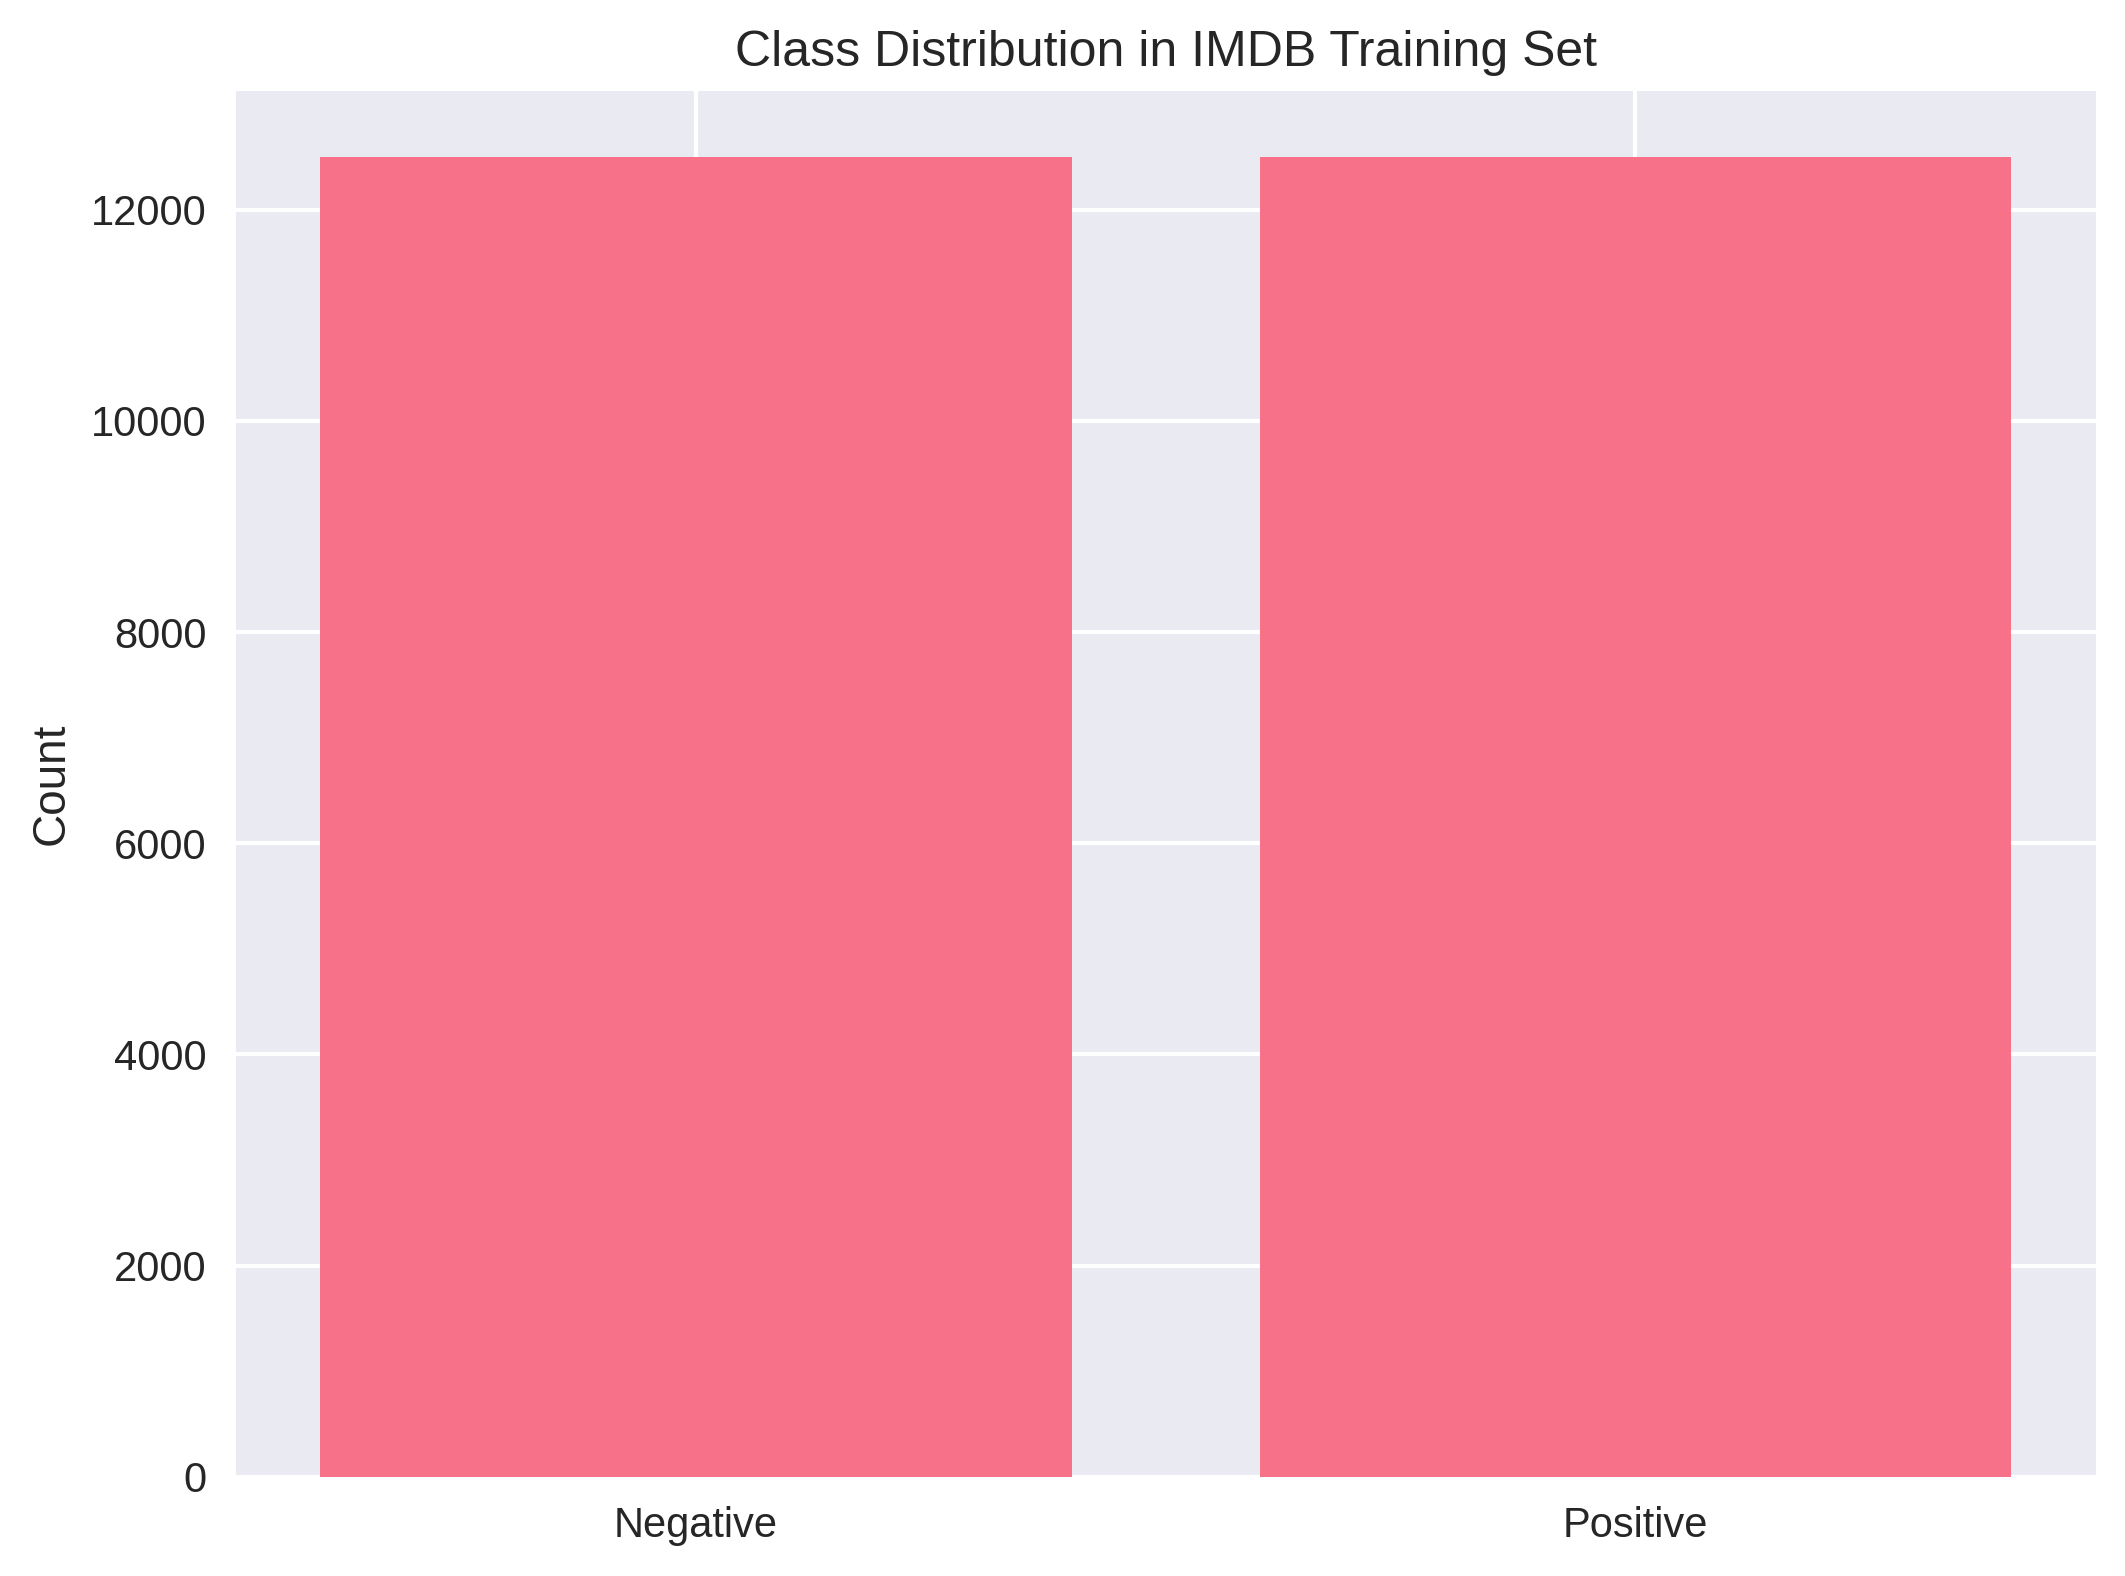
\includegraphics[width=0.75\textwidth]{../code/ch3_rnn/plots/imdb_class_distribution.png}
    \caption{Sự cân bằng dữ liệu: Biểu đồ cho thấy tập dữ liệu có số lượng mẫu Tích cực và Tiêu cực bằng nhau, lý tưởng cho việc huấn luyện mô hình phân loại.}
\end{figure}

\textbf{Giải thích chi tiết:} Biểu đồ này xác nhận dữ liệu được cân bằng giữa hai lớp, giúp giảm nguy cơ mô hình thiên vị về một lớp. Trong NLP classification, balance dataset là một điều kiện tốt để đánh giá hiệu quả mô hình thực sự.

\begin{figure}[H]
    \centering
    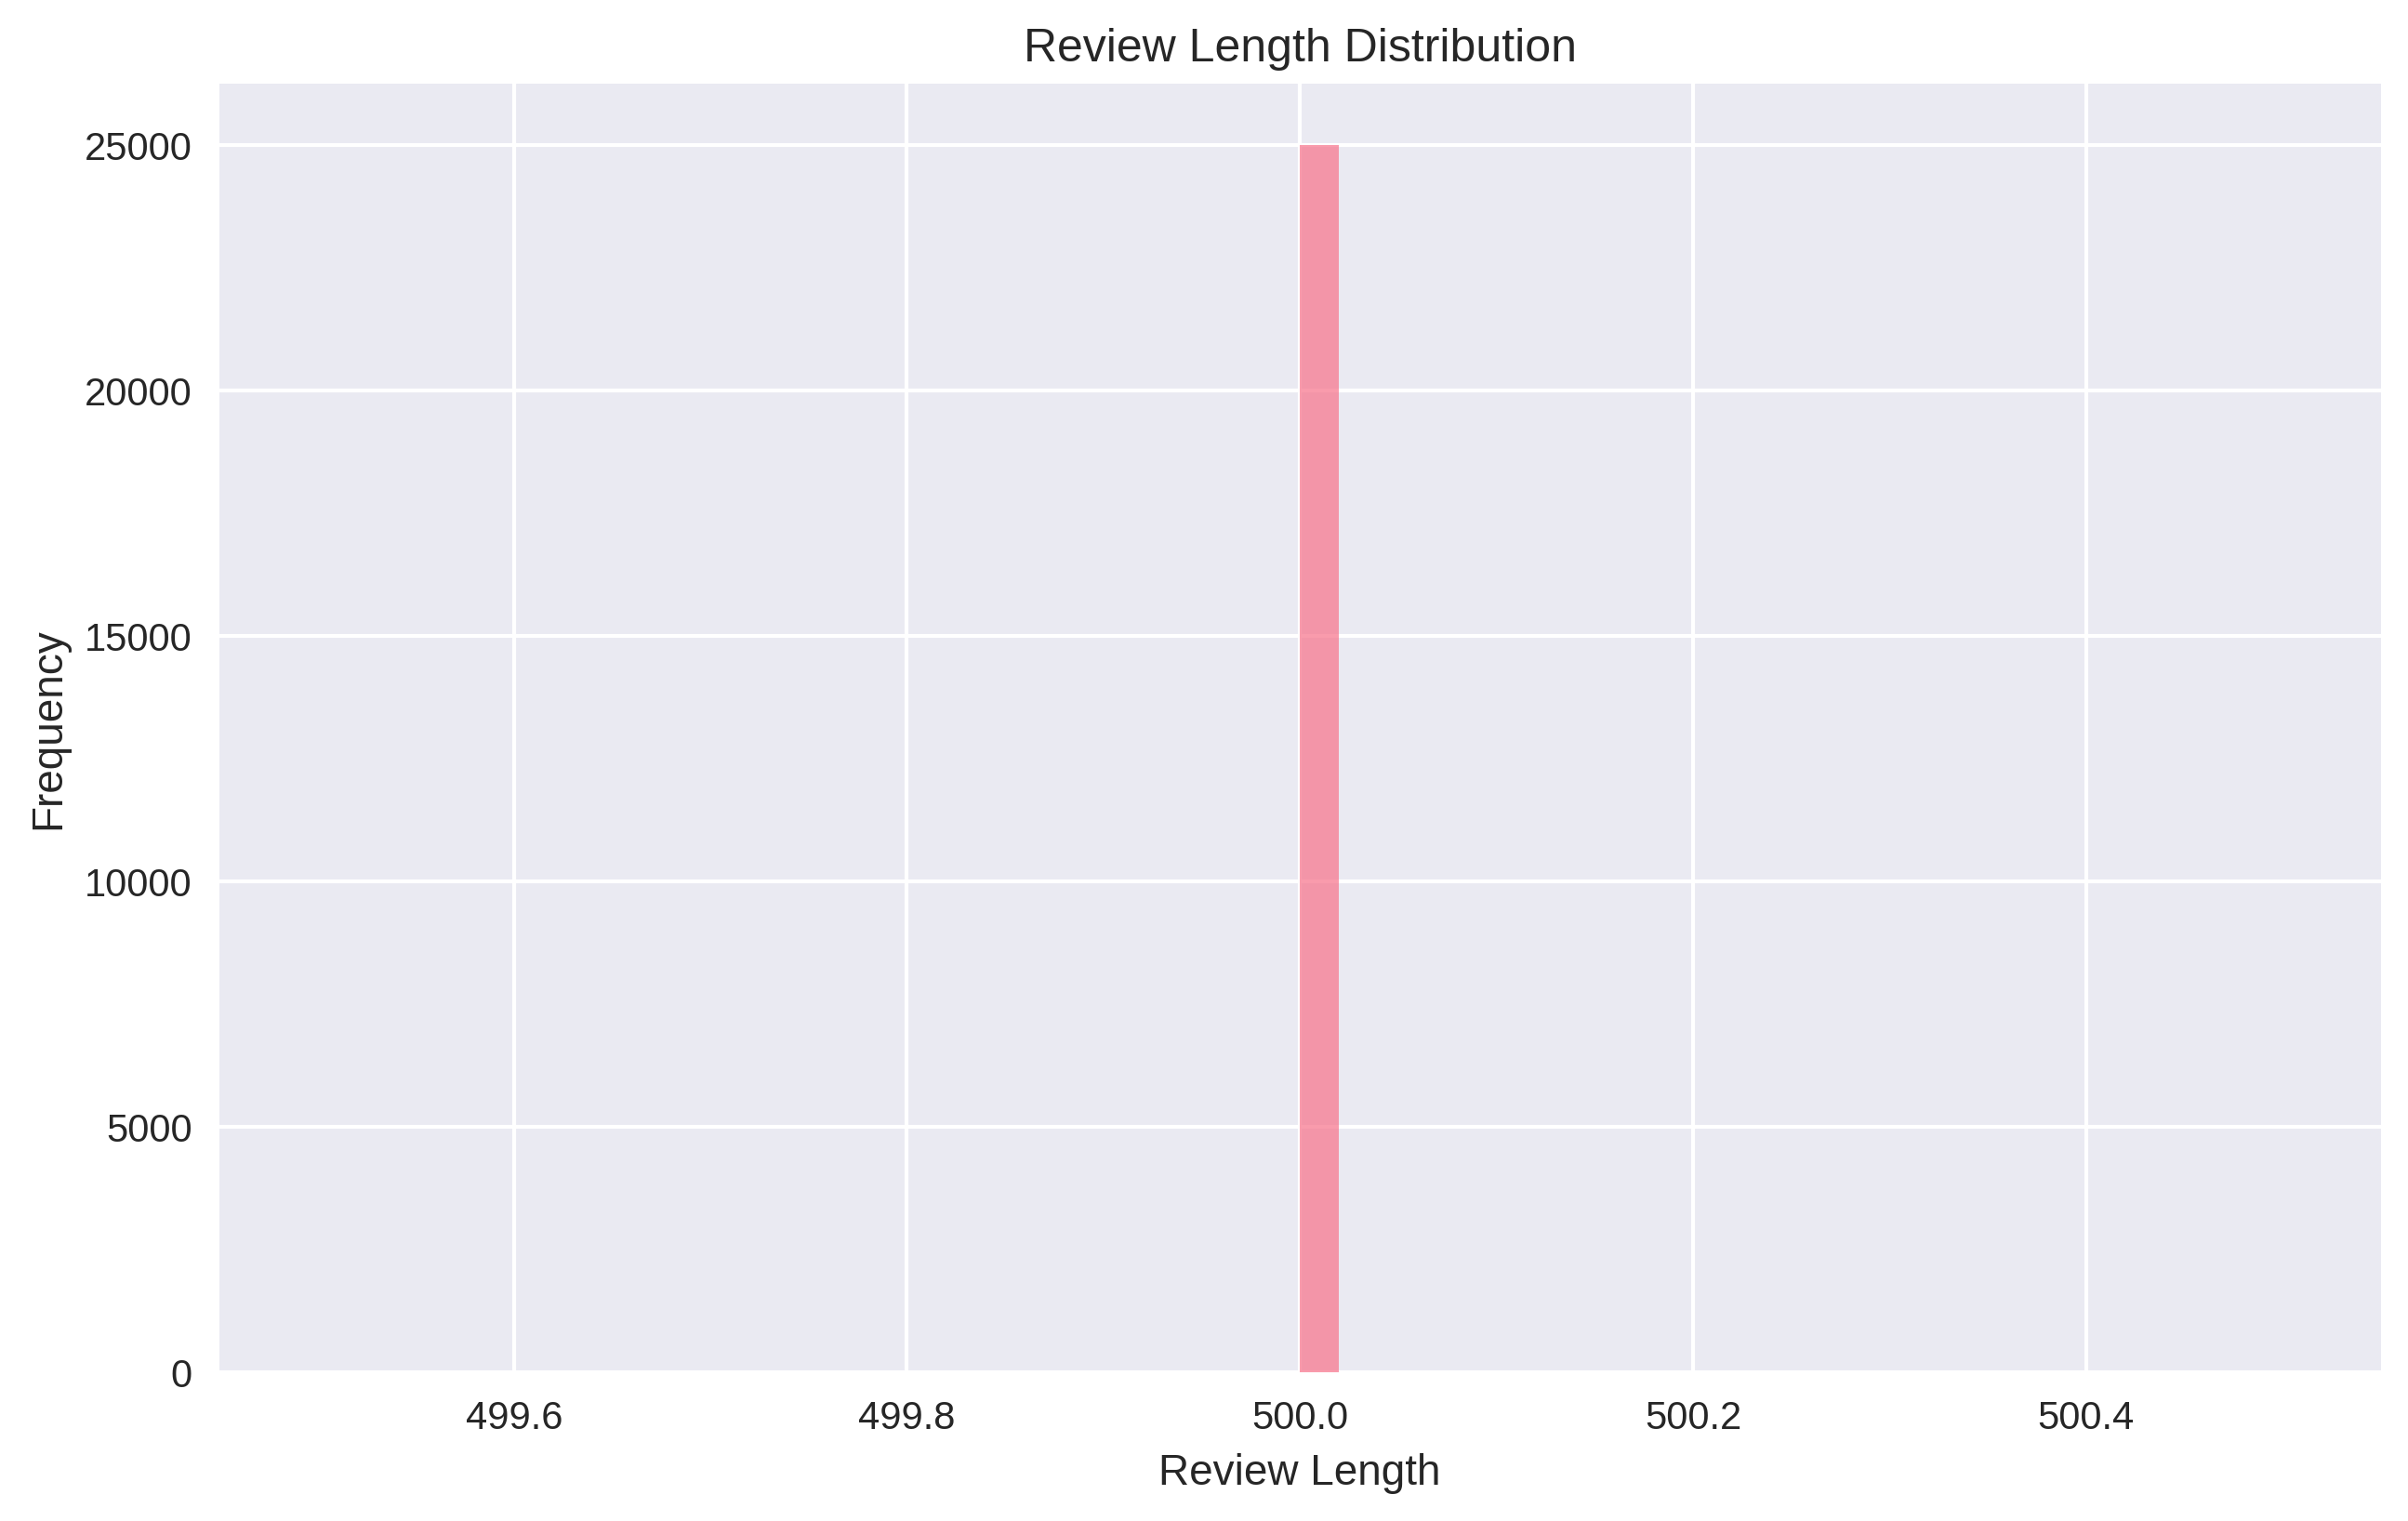
\includegraphics[width=0.75\textwidth]{../code/ch3_rnn/plots/imdb_review_length_distribution.png}
    \caption{Phân phối độ dài: Đồ thị mật độ cho thấy hầu hết các đánh giá có độ dài dưới 500 từ, đây là căn cứ để thiết lập tham số maxlen trong bước Padding.}
\end{figure}

\textbf{Giải thích chi tiết:} Dựa vào phân phối này, ta chọn maxlen phù hợp để giữ được phần lớn các review mà không lãng phí bộ nhớ. Nếu maxlen quá ngắn, mô hình có thể mất thông tin quan trọng; nếu quá dài, tập huấn luyện sẽ chậm và dễ overfit.

\begin{figure}[H]
    \centering
    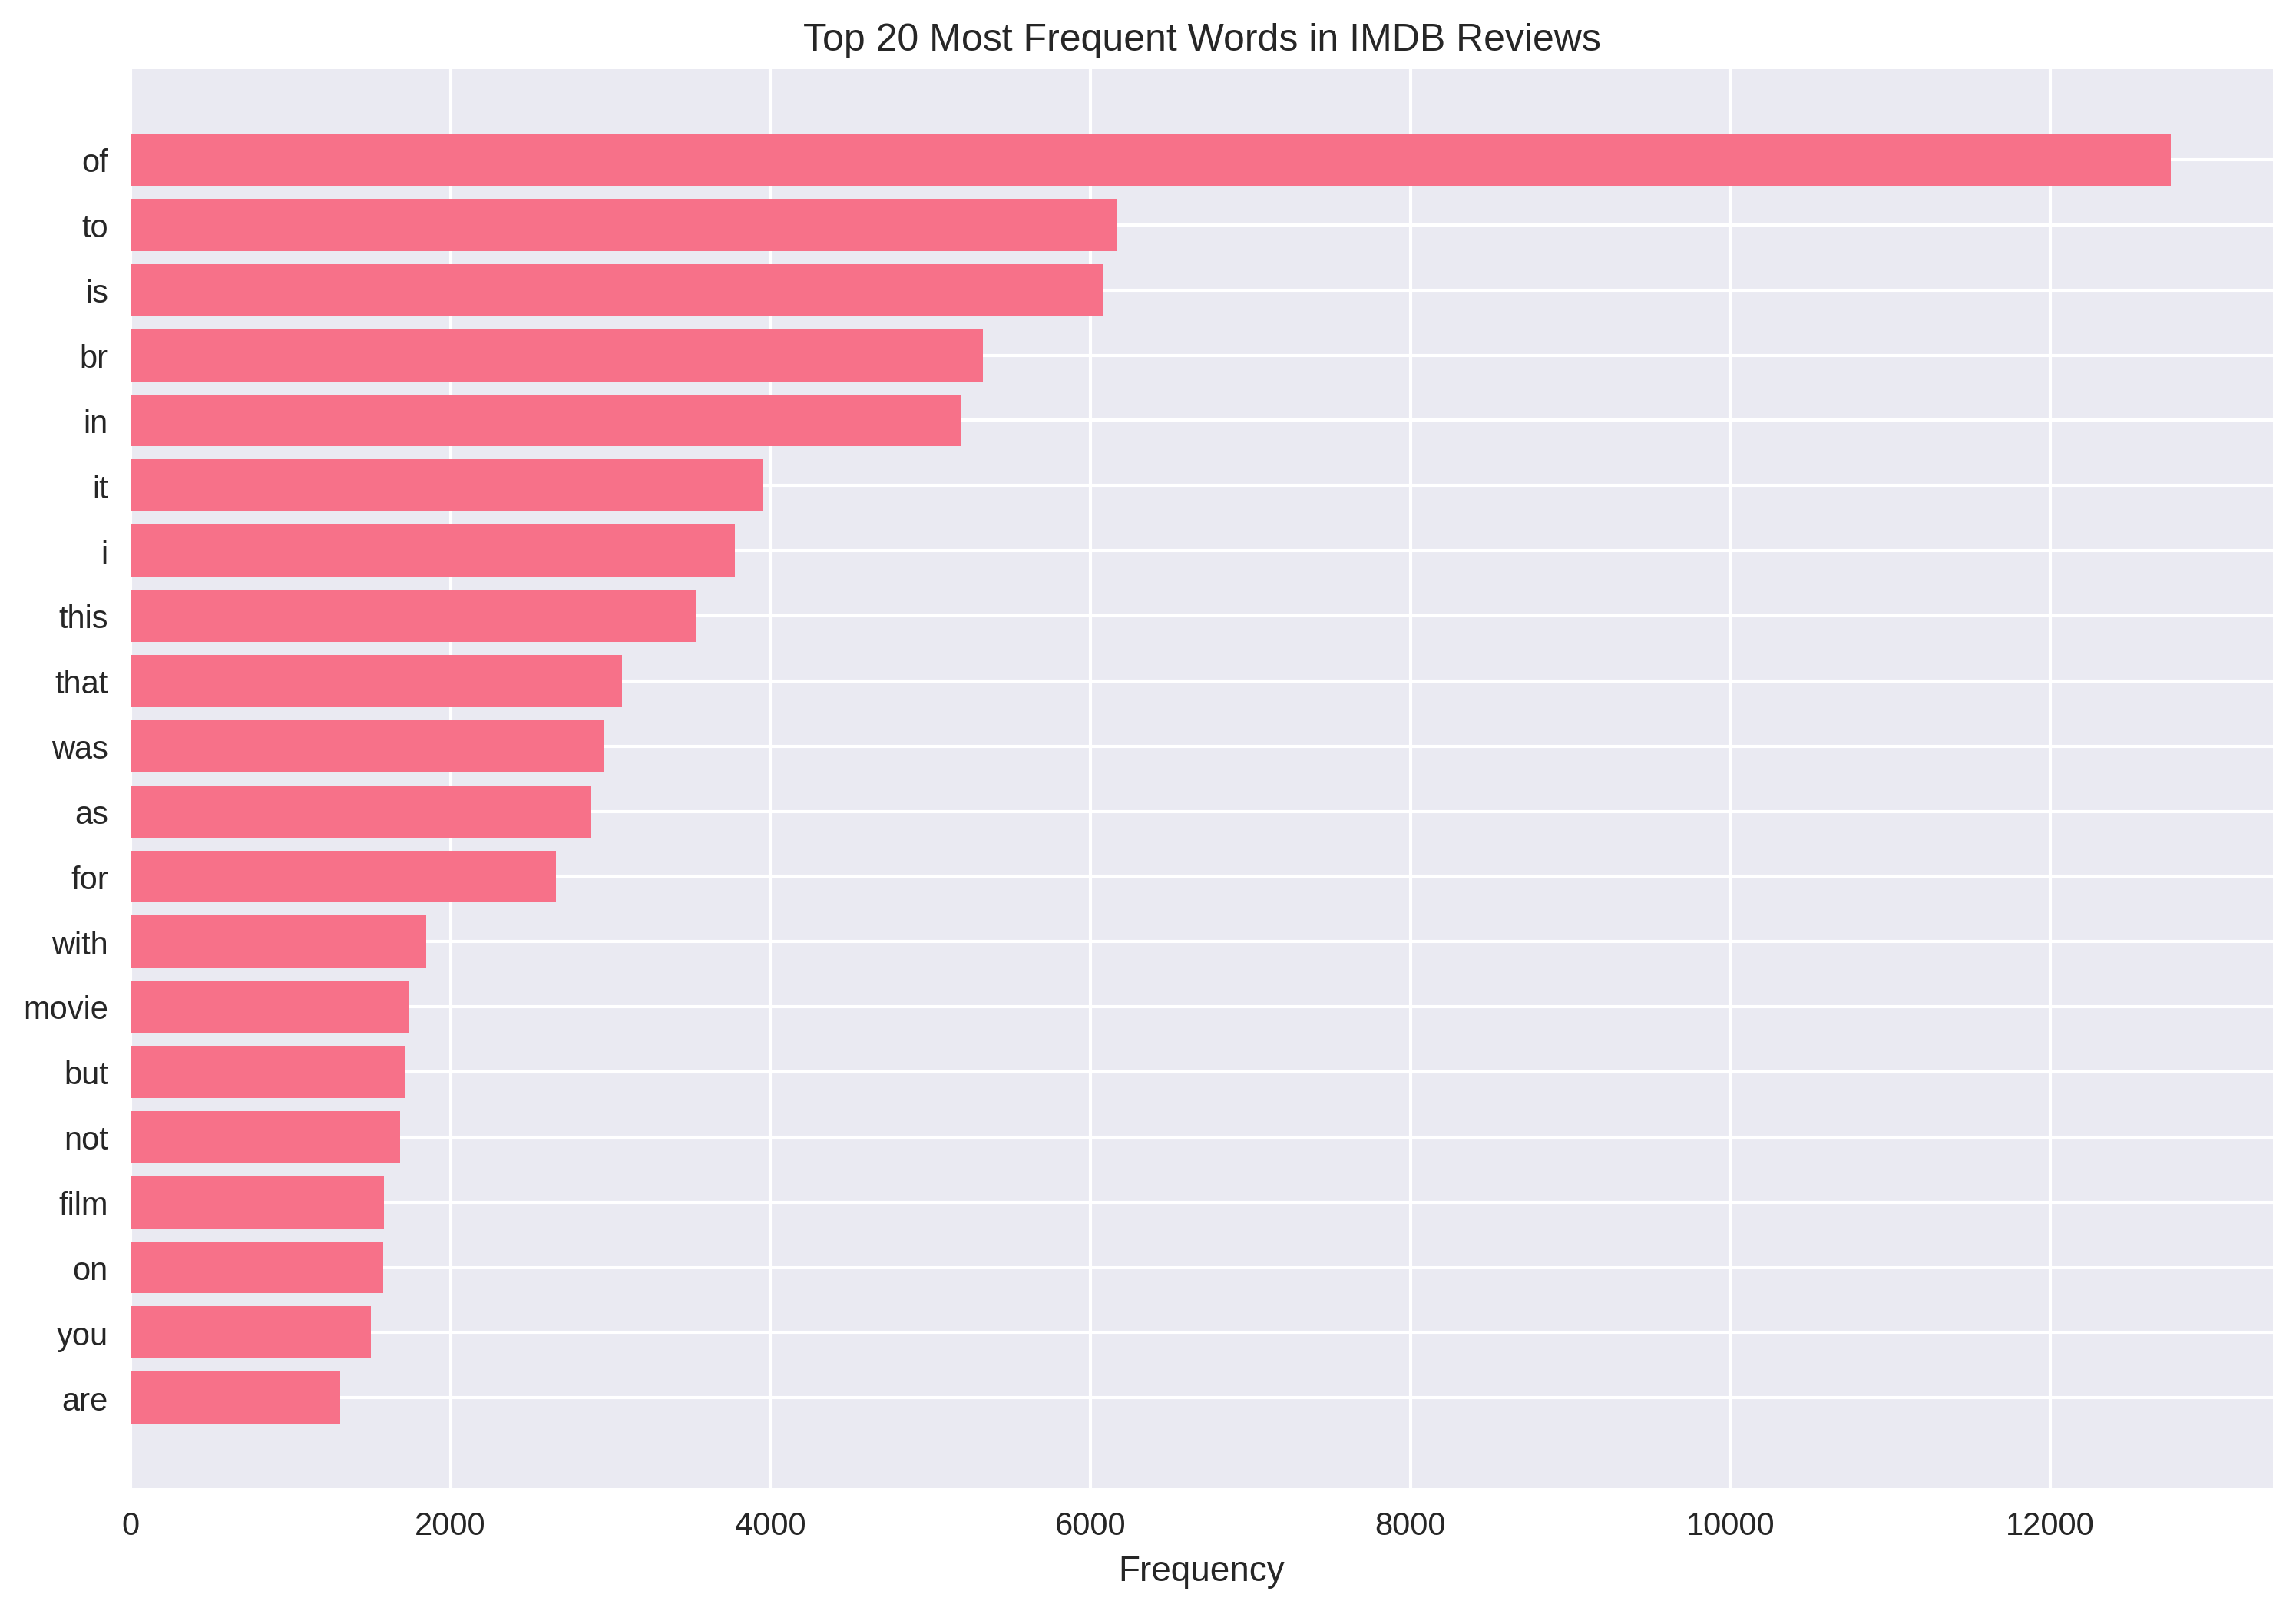
\includegraphics[width=0.75\textwidth]{../code/ch3_rnn/plots/imdb_top_words.png}
    \caption{Tần suất từ vựng: Hiển thị các từ xuất hiện nhiều nhất (đã loại bỏ stop words), phản ánh các chủ đề thường gặp trong phê bình điện ảnh.}
\end{figure}

\textbf{Giải thích chi tiết:} Biểu đồ tần suất cho thấy các từ quan trọng nhất trong dữ liệu. Loại bỏ stop words giúp mô hình tập trung vào các token mang ý nghĩa thực sự đối với phân loại cảm xúc.

Tiến hành thiết kế và huấn luyện kiến trúc RNN.

\begin{figure}[H]
    \centering
    
\includegraphics[width=0.9\textwidth]{../code/ch3_rnn/images/4.png}
    \caption{Xây dựng mạng SimpleRNN với lớp Embedding. Lớp này giúp chuyển đổi các từ đơn lẻ thành không gian vector mật độ mang ý nghĩa ngữ nghĩa.}
\end{figure}

\textbf{Giải thích chi tiết:} Embedding map mỗi từ vào một vector liên tục, cho phép học được quan hệ ngữ nghĩa giữa các từ. SimpleRNN giữ được trạng thái ẩn của chuỗi để thể hiện ngữ cảnh từng câu.

\textbf{Cơ chế Hidden State:} Lớp \texttt{SimpleRNN} chính là nơi hiện thực hóa công thức tính $h_t$ (mục 3.2.2). Tại đây, mạng duy trì một vòng lặp nội tại để lưu trữ thông tin của các từ đứng trước, giúp mô hình "hiểu" được ngữ cảnh của cả câu văn thay vì chỉ nhìn vào từng từ độc lập.

\begin{figure}[H]
    \centering
    
\includegraphics[width=0.9\textwidth]{../code/ch3_rnn/images/5.png}
    \caption{Triển khai quá trình huấn luyện: Sử dụng Dropout để giảm thiểu hiện tượng Overfitting - một vấn đề phổ biến khi huấn luyện trên dữ liệu văn bản phức tạp.}
\end{figure}

\textbf{Giải thích chi tiết:} Dropout ngẫu nhiên loại bỏ một phần đơn vị trong mạng khi huấn luyện, giúp giảm khả năng mạng học quá kỹ những mẫu huấn luyện và cải thiện generalization trên dữ liệu mới.

\begin{figure}[H]
    \centering
    
\includegraphics[width=0.9\textwidth]{../code/ch3_rnn/images/6.png}
    \caption{Nâng cấp mô hình với Bidirectional RNN: Cho phép mạng học thông tin từ cả hai hướng (quá khứ và tương lai), giúp nắm bắt ngữ cảnh tốt hơn.}
\end{figure}

\textbf{Giải thích chi tiết:} Bidirectional RNN đọc chuỗi cả theo chiều xuôi và ngược, cho phép mô hình sử dụng cả thông tin phía trước và phía sau của mỗi token. Điều này đặc biệt hữu ích với văn bản, nơi nghĩa phụ thuộc vào ngữ cảnh trước và sau.

\textbf{Phân tích Bidirectional:} Theo lý thuyết ở mục 3.6.2, việc sử dụng kiến trúc hai chiều giúp trạng thái ẩn $h_t$ tại mỗi bước thời gian tổng hợp được thông tin từ cả đầu chuỗi và cuối chuỗi. Điều này cực kỳ hữu ích trong NLP, nơi nghĩa của một từ thường phụ thuộc vào các từ xuất hiện sau nó.

\begin{figure}[H]
    \centering
    
\includegraphics[width=0.9\textwidth]{../code/ch3_rnn/images/7.png}
    \caption{Xây dựng hàm suy diễn (Inference): Cho phép người dùng nhập một câu văn bất kỳ và mô hình sẽ trả về dự đoán xác suất cảm xúc.}
\end{figure}

\textbf{Giải thích chi tiết:} Hàm inference chuyển đổi văn bản mới thành cùng định dạng input, rồi dùng mô hình đã huấn luyện để dự đoán. Đây là bước cần thiết để đưa mô hình từ phòng thí nghiệm vào ứng dụng thực tế.

Đánh giá kết quả mô hình IMDB:

\begin{figure}[H]
    \centering
    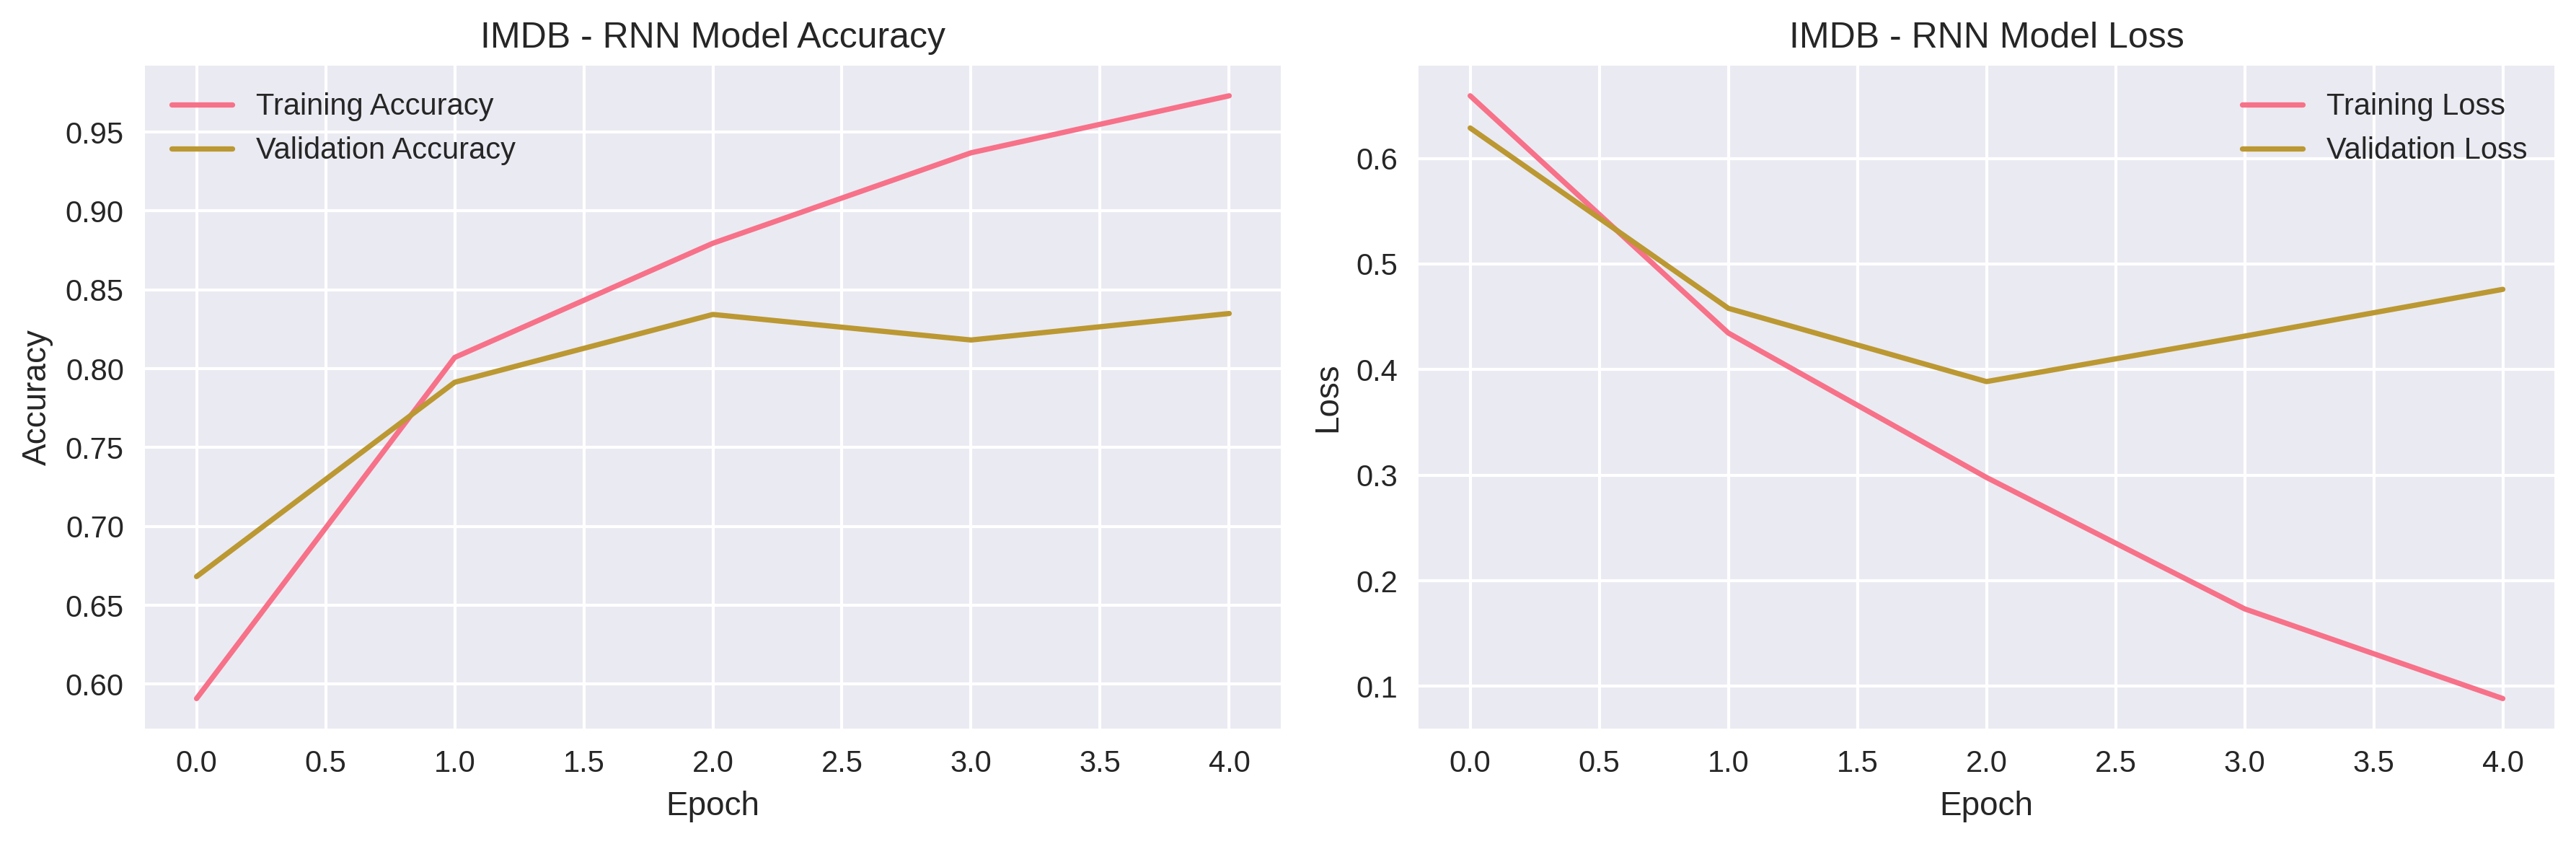
\includegraphics[width=0.75\textwidth]{../code/ch3_rnn/plots/imdb_rnn_training_history.png}
    \caption{Lịch sử huấn luyện: Quan sát sự phân kỳ giữa Training Accuracy và Validation Accuracy để xác định điểm dừng tối ưu tránh quá khớp.}
\end{figure}

\textbf{Giải thích chi tiết:} Sự phân kỳ giữa training và validation cho thấy mô hình bắt đầu overfit. Nếu validation accuracy giảm trong khi training accuracy vẫn tăng, ta cần dừng sớm hoặc tăng regularization.

\textbf{Hiện tượng Overfitting:} Biểu đồ trên minh chứng cho lý thuyết ở mục 3.10. Sự phân kỳ giữa hai đường Accuracy sau Epoch thứ 4 cho thấy mô hình bắt đầu "học thuộc lòng" tập huấn luyện thay vì học quy luật chung, đòi hỏi chúng ta phải áp dụng Early Stopping hoặc tăng cường Dropout.

\begin{figure}[H]
    \centering
    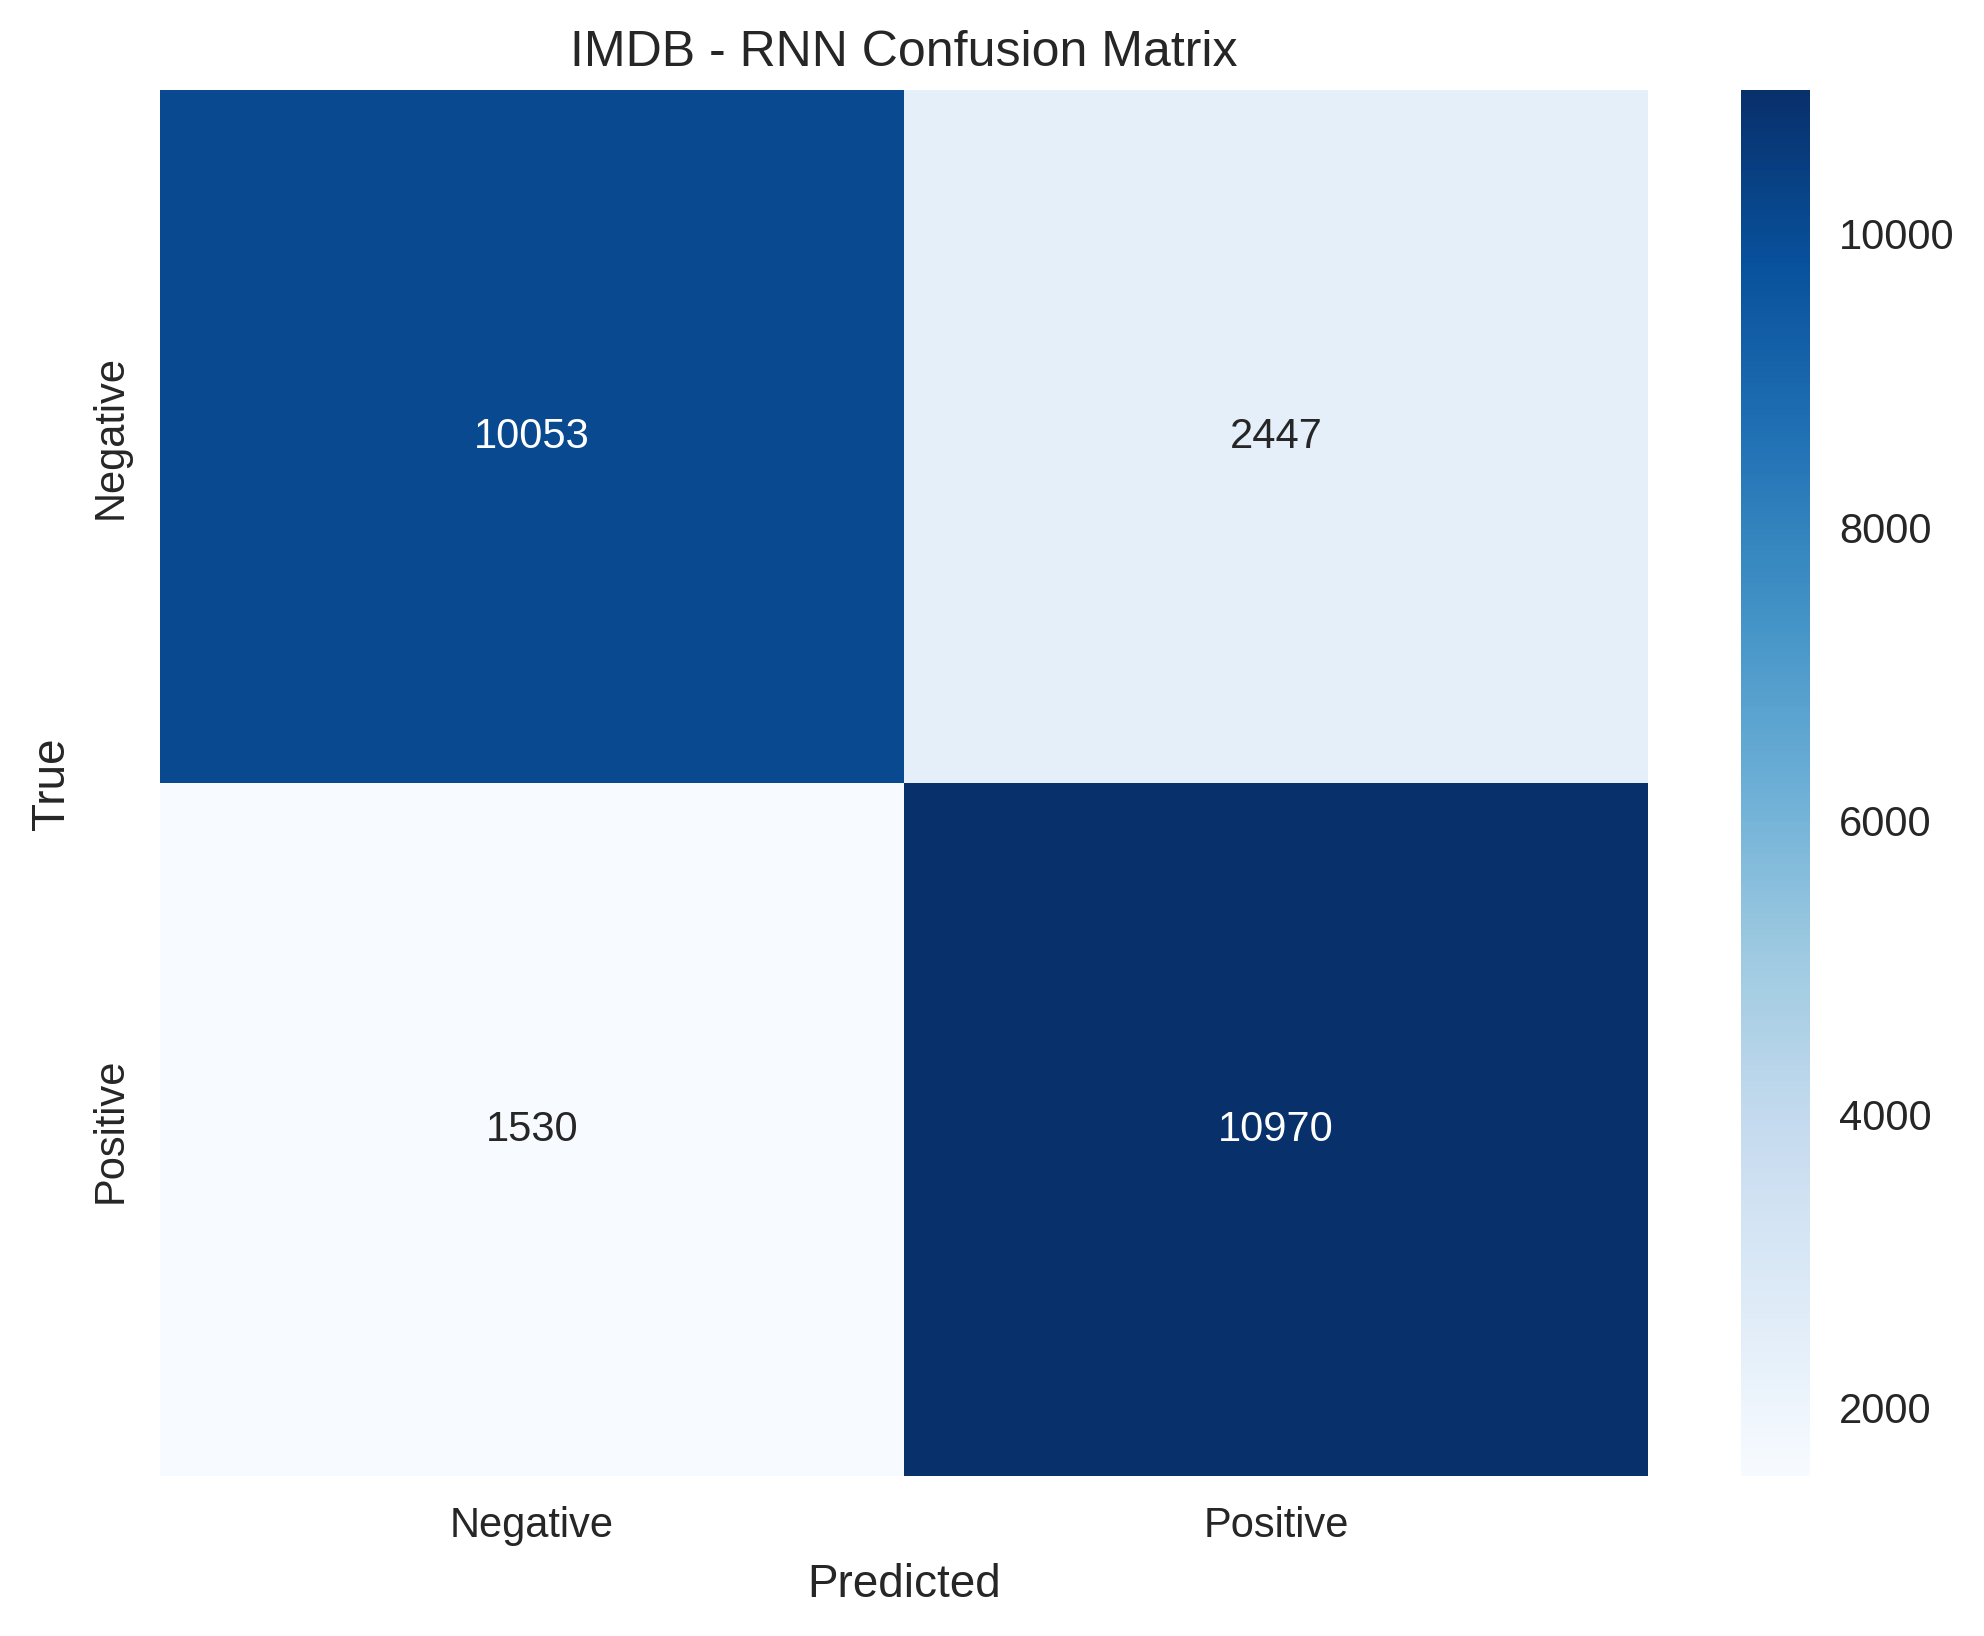
\includegraphics[width=0.75\textwidth]{../code/ch3_rnn/plots/imdb_rnn_confusion_matrix.png}
    \caption{Ma trận nhầm lẫn: Thể hiện độ chính xác của mô hình trên tập Test, chỉ rõ số lượng mẫu bị dự đoán sai giữa hai lớp.}
\end{figure}

\textbf{Giải thích chi tiết:} Confusion matrix giúp phân tích chi tiết các lỗi dự đoán: false positive và false negative. Với bài toán sentiment, hiểu loại lỗi này quan trọng để điều chỉnh mô hình theo mục tiêu bài toán.

\subsubsection{Bài toán 2: Dự đoán chuỗi Sine Wave}
Bài toán này kiểm tra khả năng học các quy luật tuần hoàn và dự báo các giá trị liên tục trong tương lai của RNN.

\begin{figure}[H]
    \centering
    
\includegraphics[width=0.9\textwidth]{../code/ch3_rnn/images/8.png}
    \caption{Sinh dữ liệu nhân tạo: Tạo sóng hình sin có kèm nhiễu trắng để mô phỏng dữ liệu chuỗi thời gian thực tế.}
\end{figure}

\textbf{Giải thích chi tiết:} Quá trình sinh dữ liệu nhân tạo cho phép chúng ta kiểm soát hoàn toàn các thuộc tính của chuỗi thời gian như tần số, biên độ và mức độ nhiễu. Việc thêm nhiễu trắng (Gaussian Noise) là cần thiết để mô phỏng tính không chắc chắn của dữ liệu thực tế, buộc RNN phải học cách lọc nhiễu để tìm ra quy luật cốt lõi.

\begin{figure}[H]
    \centering
    
\includegraphics[width=0.9\textwidth]{../code/ch3_rnn/images/9.png}
    \caption{Mã nguồn EDA cho Sine Wave: Trực quan hóa cấu trúc sóng và phân tích tính tự tương quan (Autocorrelation).}
\end{figure}

\textbf{Giải thích chi tiết:} EDA với autocorrelation giúp xác định độ trễ tối ưu cho dự báo. Nếu chuỗi có độ tự tương quan cao ở lag nhất định, mô hình có thể học tốt quy luật tuần hoàn dựa trên các giá trị lịch sử lặp lại.

Các phân tích đặc trưng Sine Wave:

\begin{figure}[H]
    \centering
    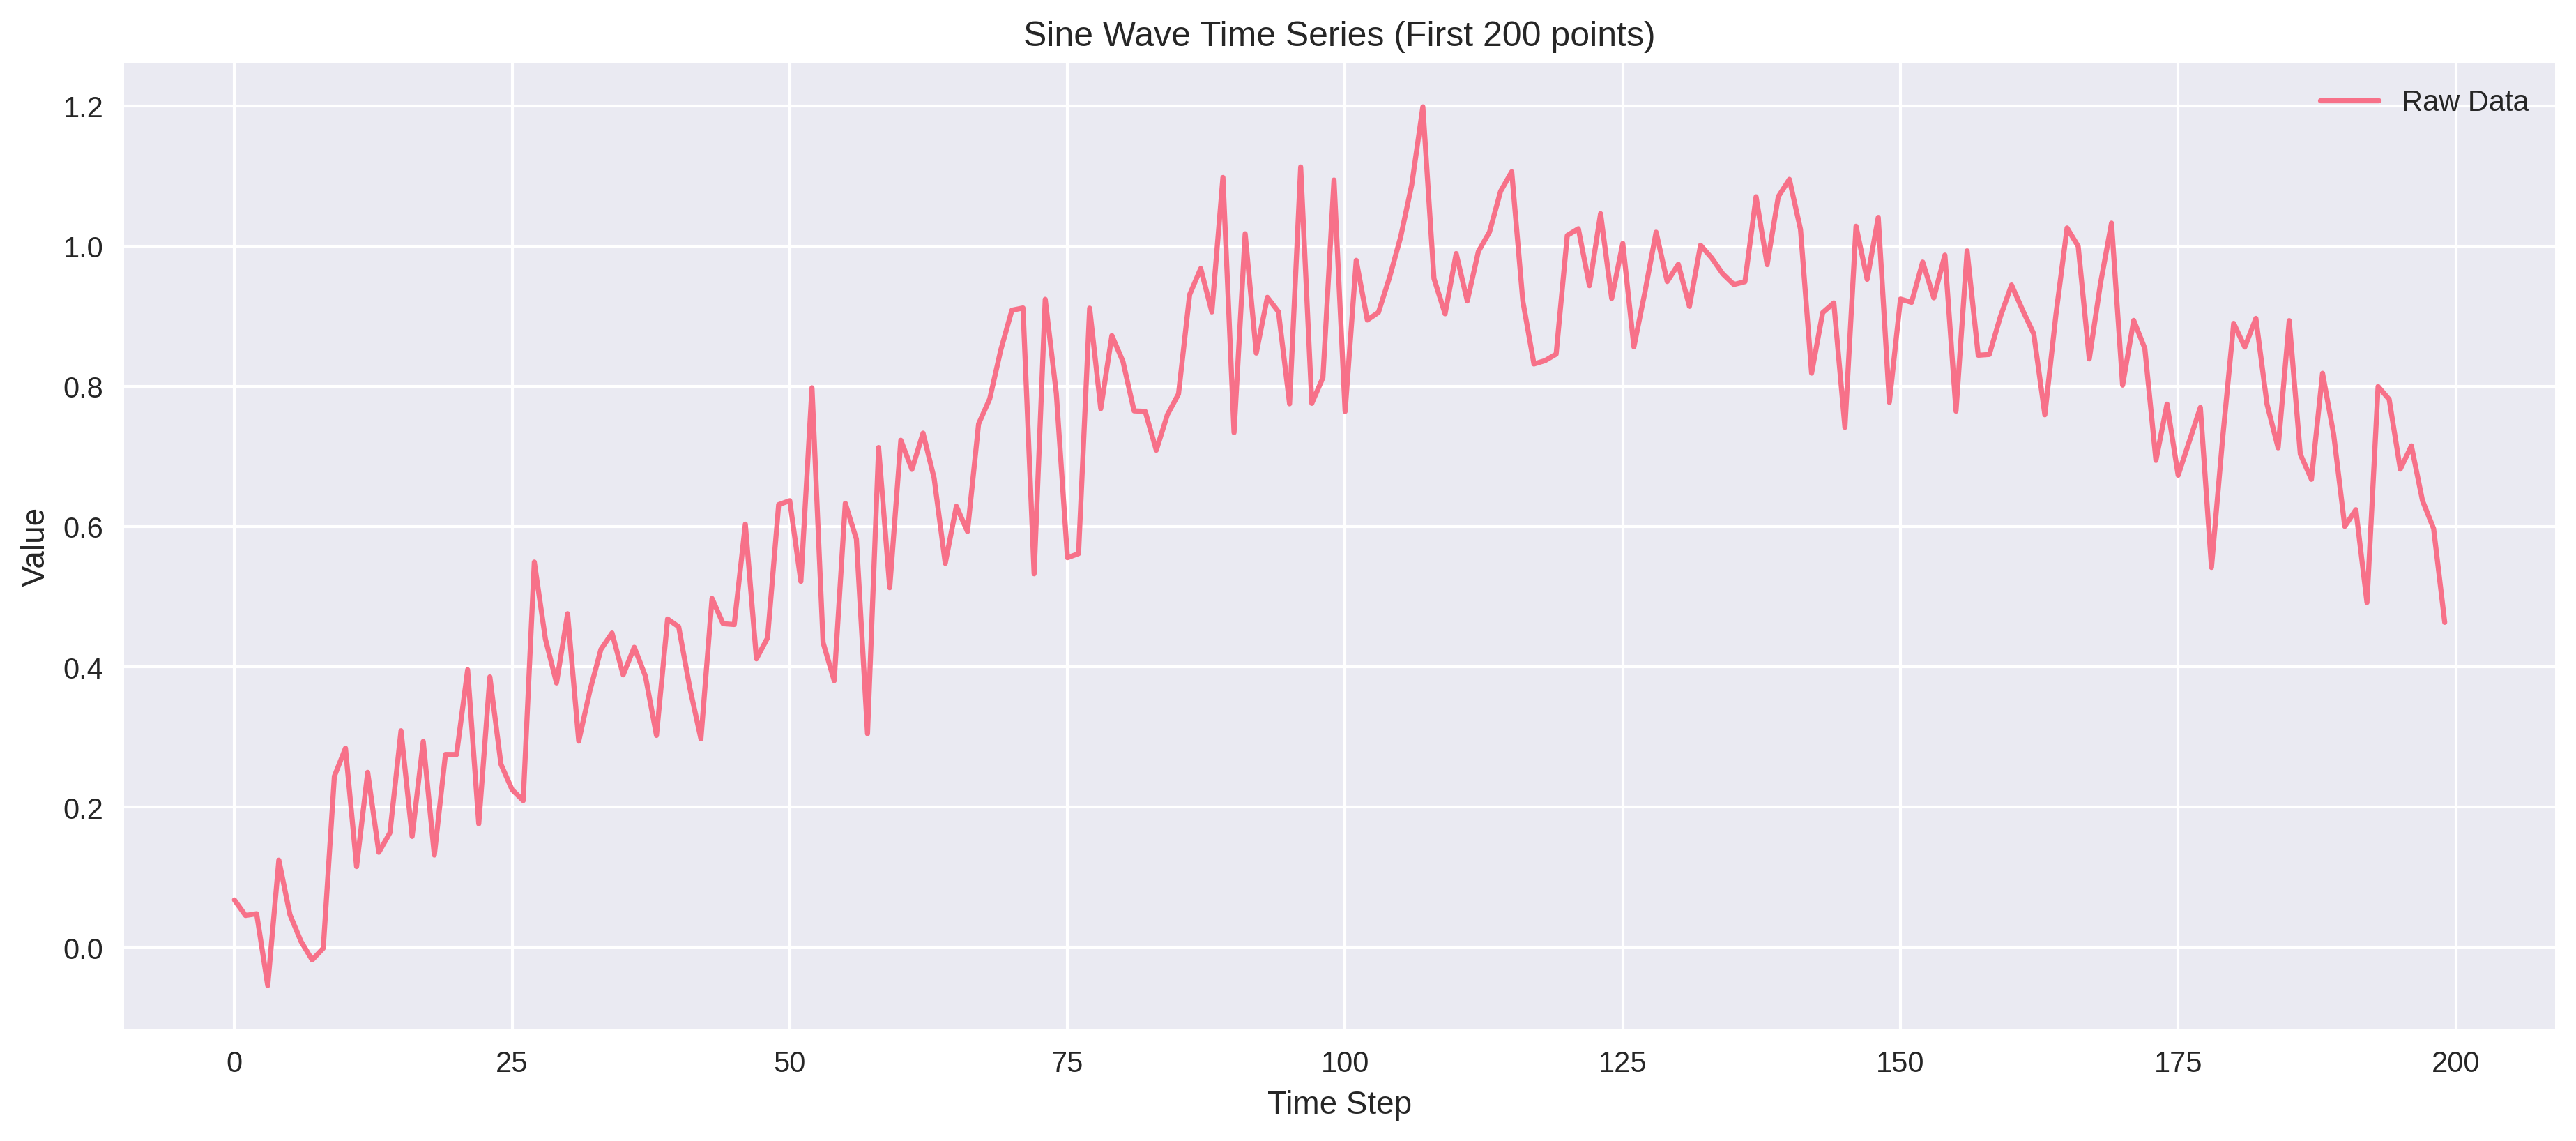
\includegraphics[width=0.75\textwidth]{../code/ch3_rnn/plots/sine_wave_raw_data.png}
    \caption{Dữ liệu thô: Biểu đồ chuỗi thời gian cho thấy tính chu kỳ rõ rệt của hàm Sine mặc dù có nhiễu.}
\end{figure}

\textbf{Giải thích chi tiết:} Biểu đồ chuỗi thời gian thô xác nhận dữ liệu có tính ổn định về mặt thống kê (stationary) sau khi loại bỏ nhiễu. Tính tuần hoàn rõ rệt là dấu hiệu cho thấy một mạng RNN cơ bản có thể học được quy luật mà không cần đến các kiến trúc phức tạp hơn như Transformer.

\begin{figure}[H]
    \centering
    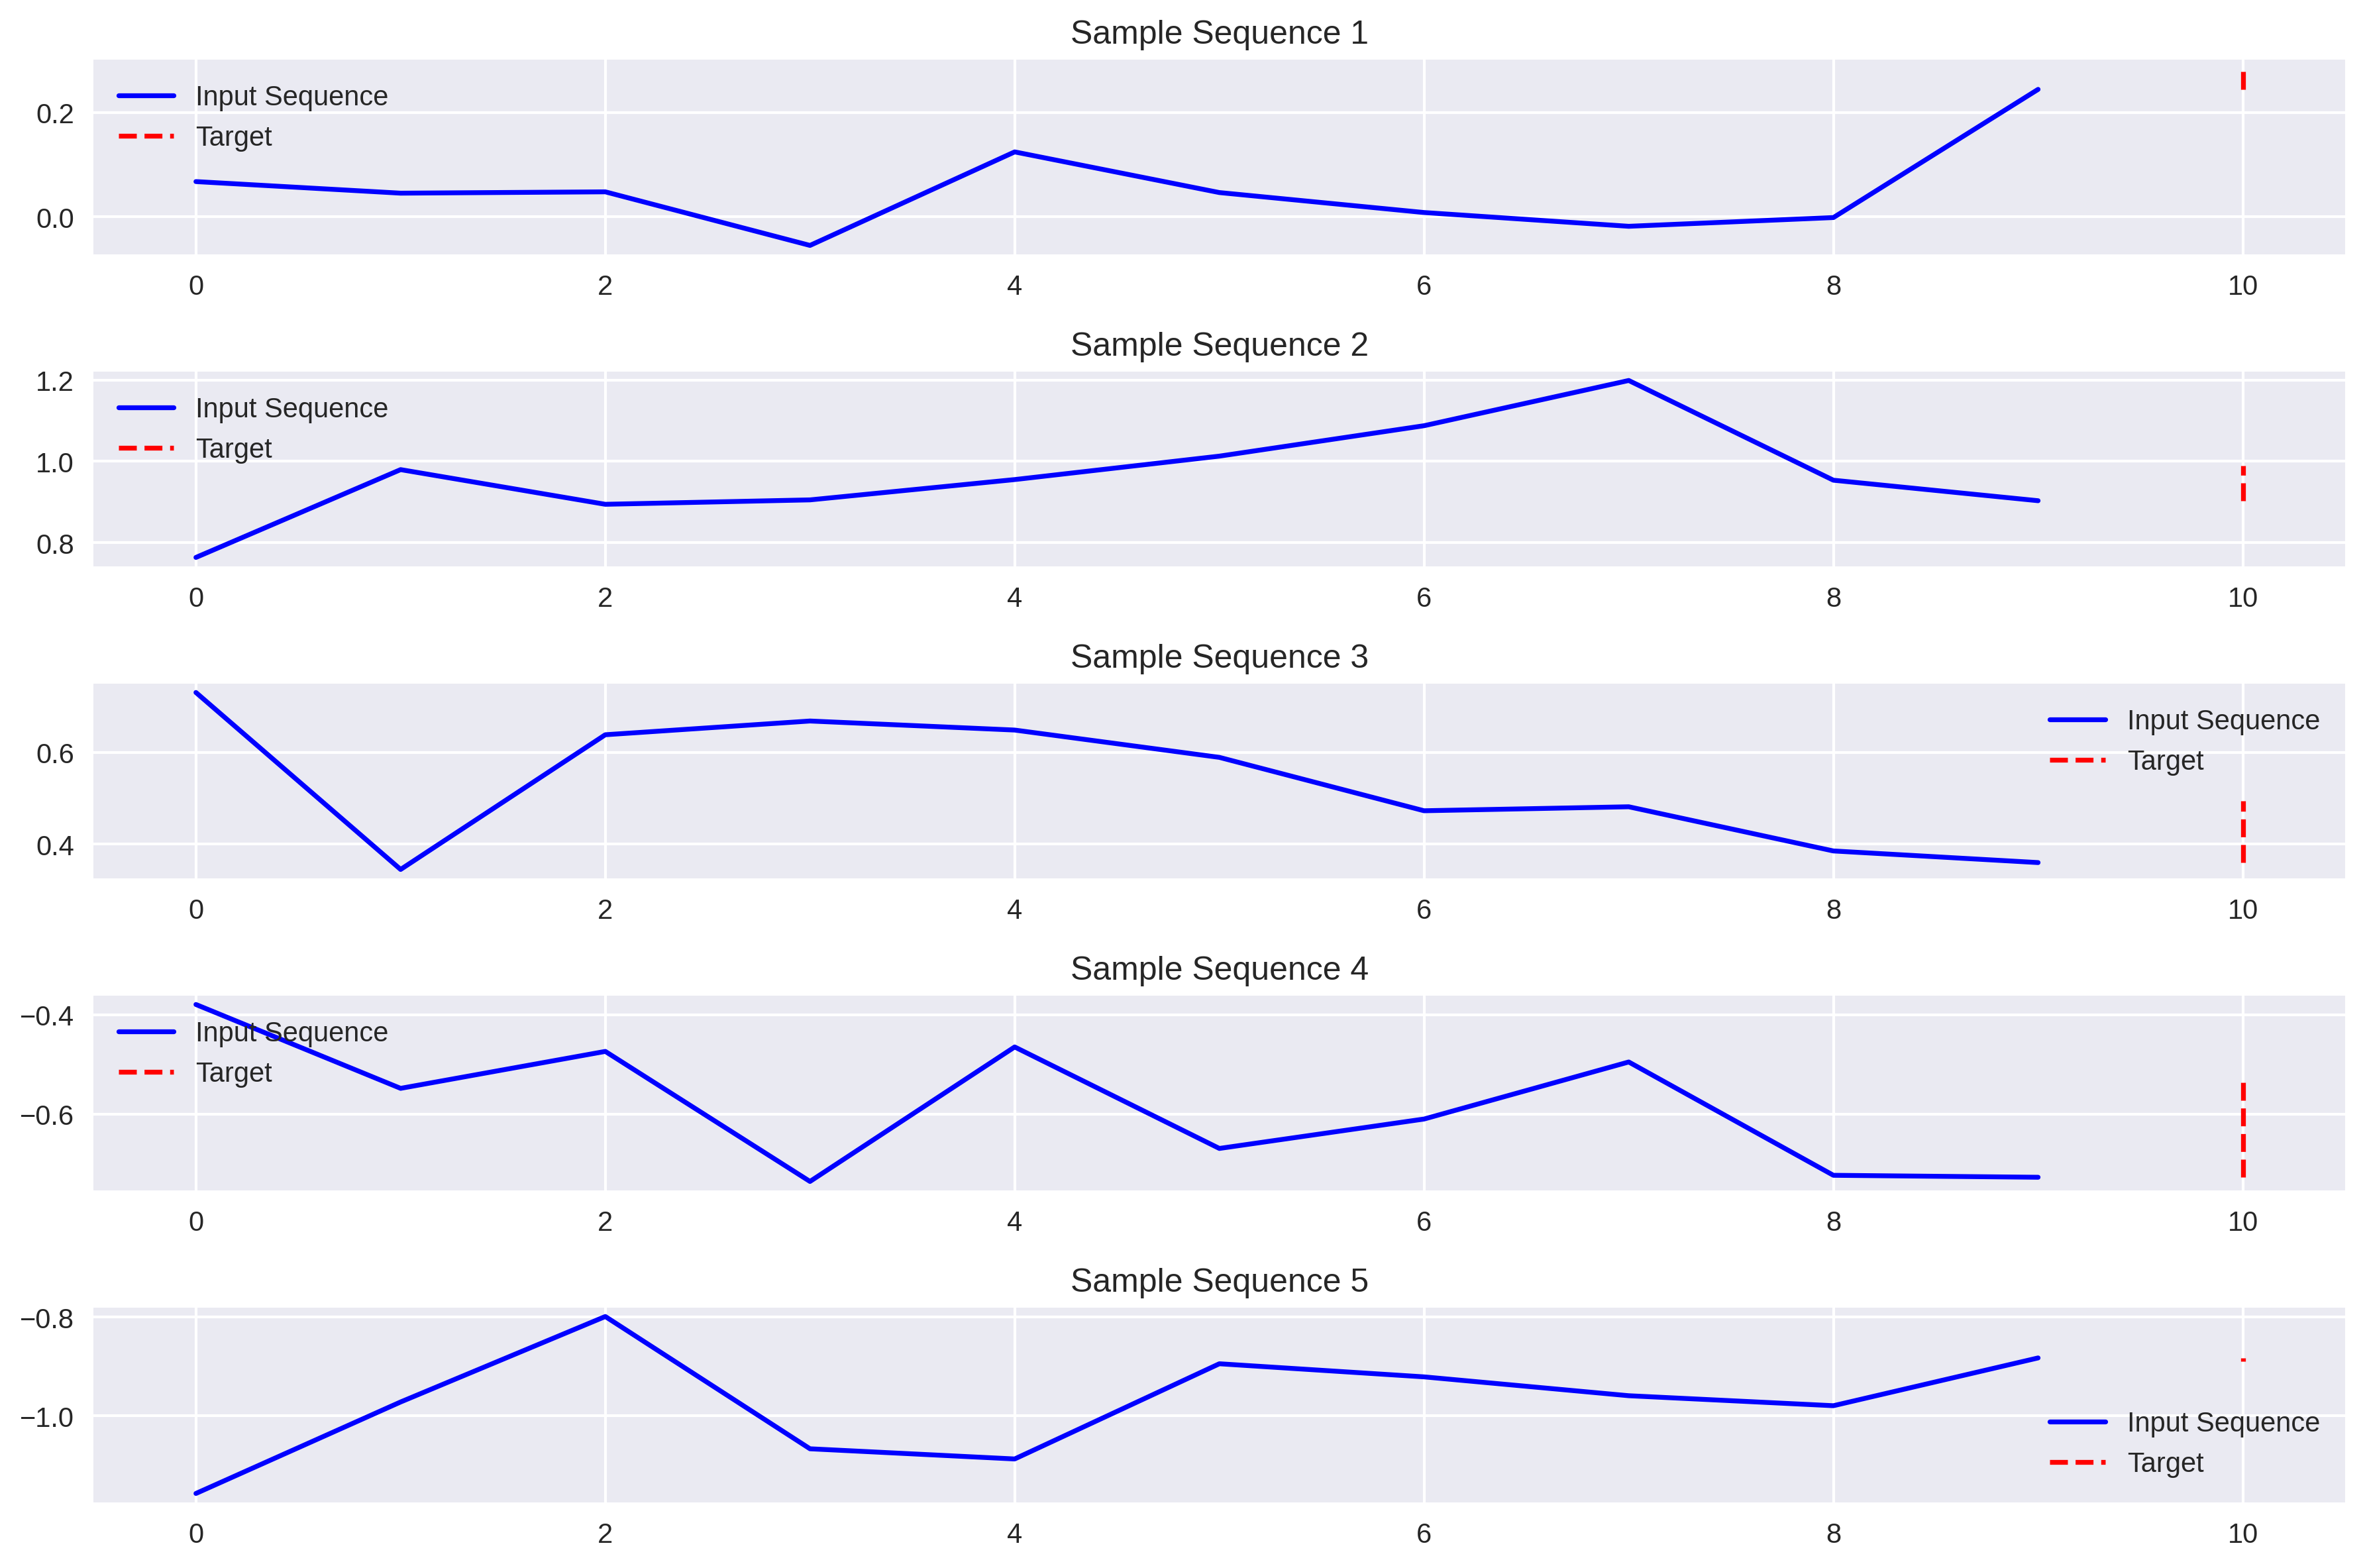
\includegraphics[width=0.75\textwidth]{../code/ch3_rnn/plots/sine_wave_sample_sequences.png}
    \caption{Mẫu cửa sổ trượt: Hiển thị cách dữ liệu được chia thành các đoạn nhỏ (Time Steps) để đưa vào mô hình RNN.}
\end{figure}

\textbf{Giải thích chi tiết:} Kỹ thuật cửa sổ trượt (Sliding Window) chuyển đổi dữ liệu chuỗi đơn lẻ thành tập dữ liệu giám sát. Mỗi cửa sổ chứa $n$ bước thời gian quá khứ làm đầu vào ($X$) để dự báo giá trị tại bước $t+1$ làm nhãn ($y$). Đây là bước chuẩn bị dữ liệu quan trọng nhất trong học sâu cho chuỗi thời gian.

\begin{figure}[H]
    \centering
    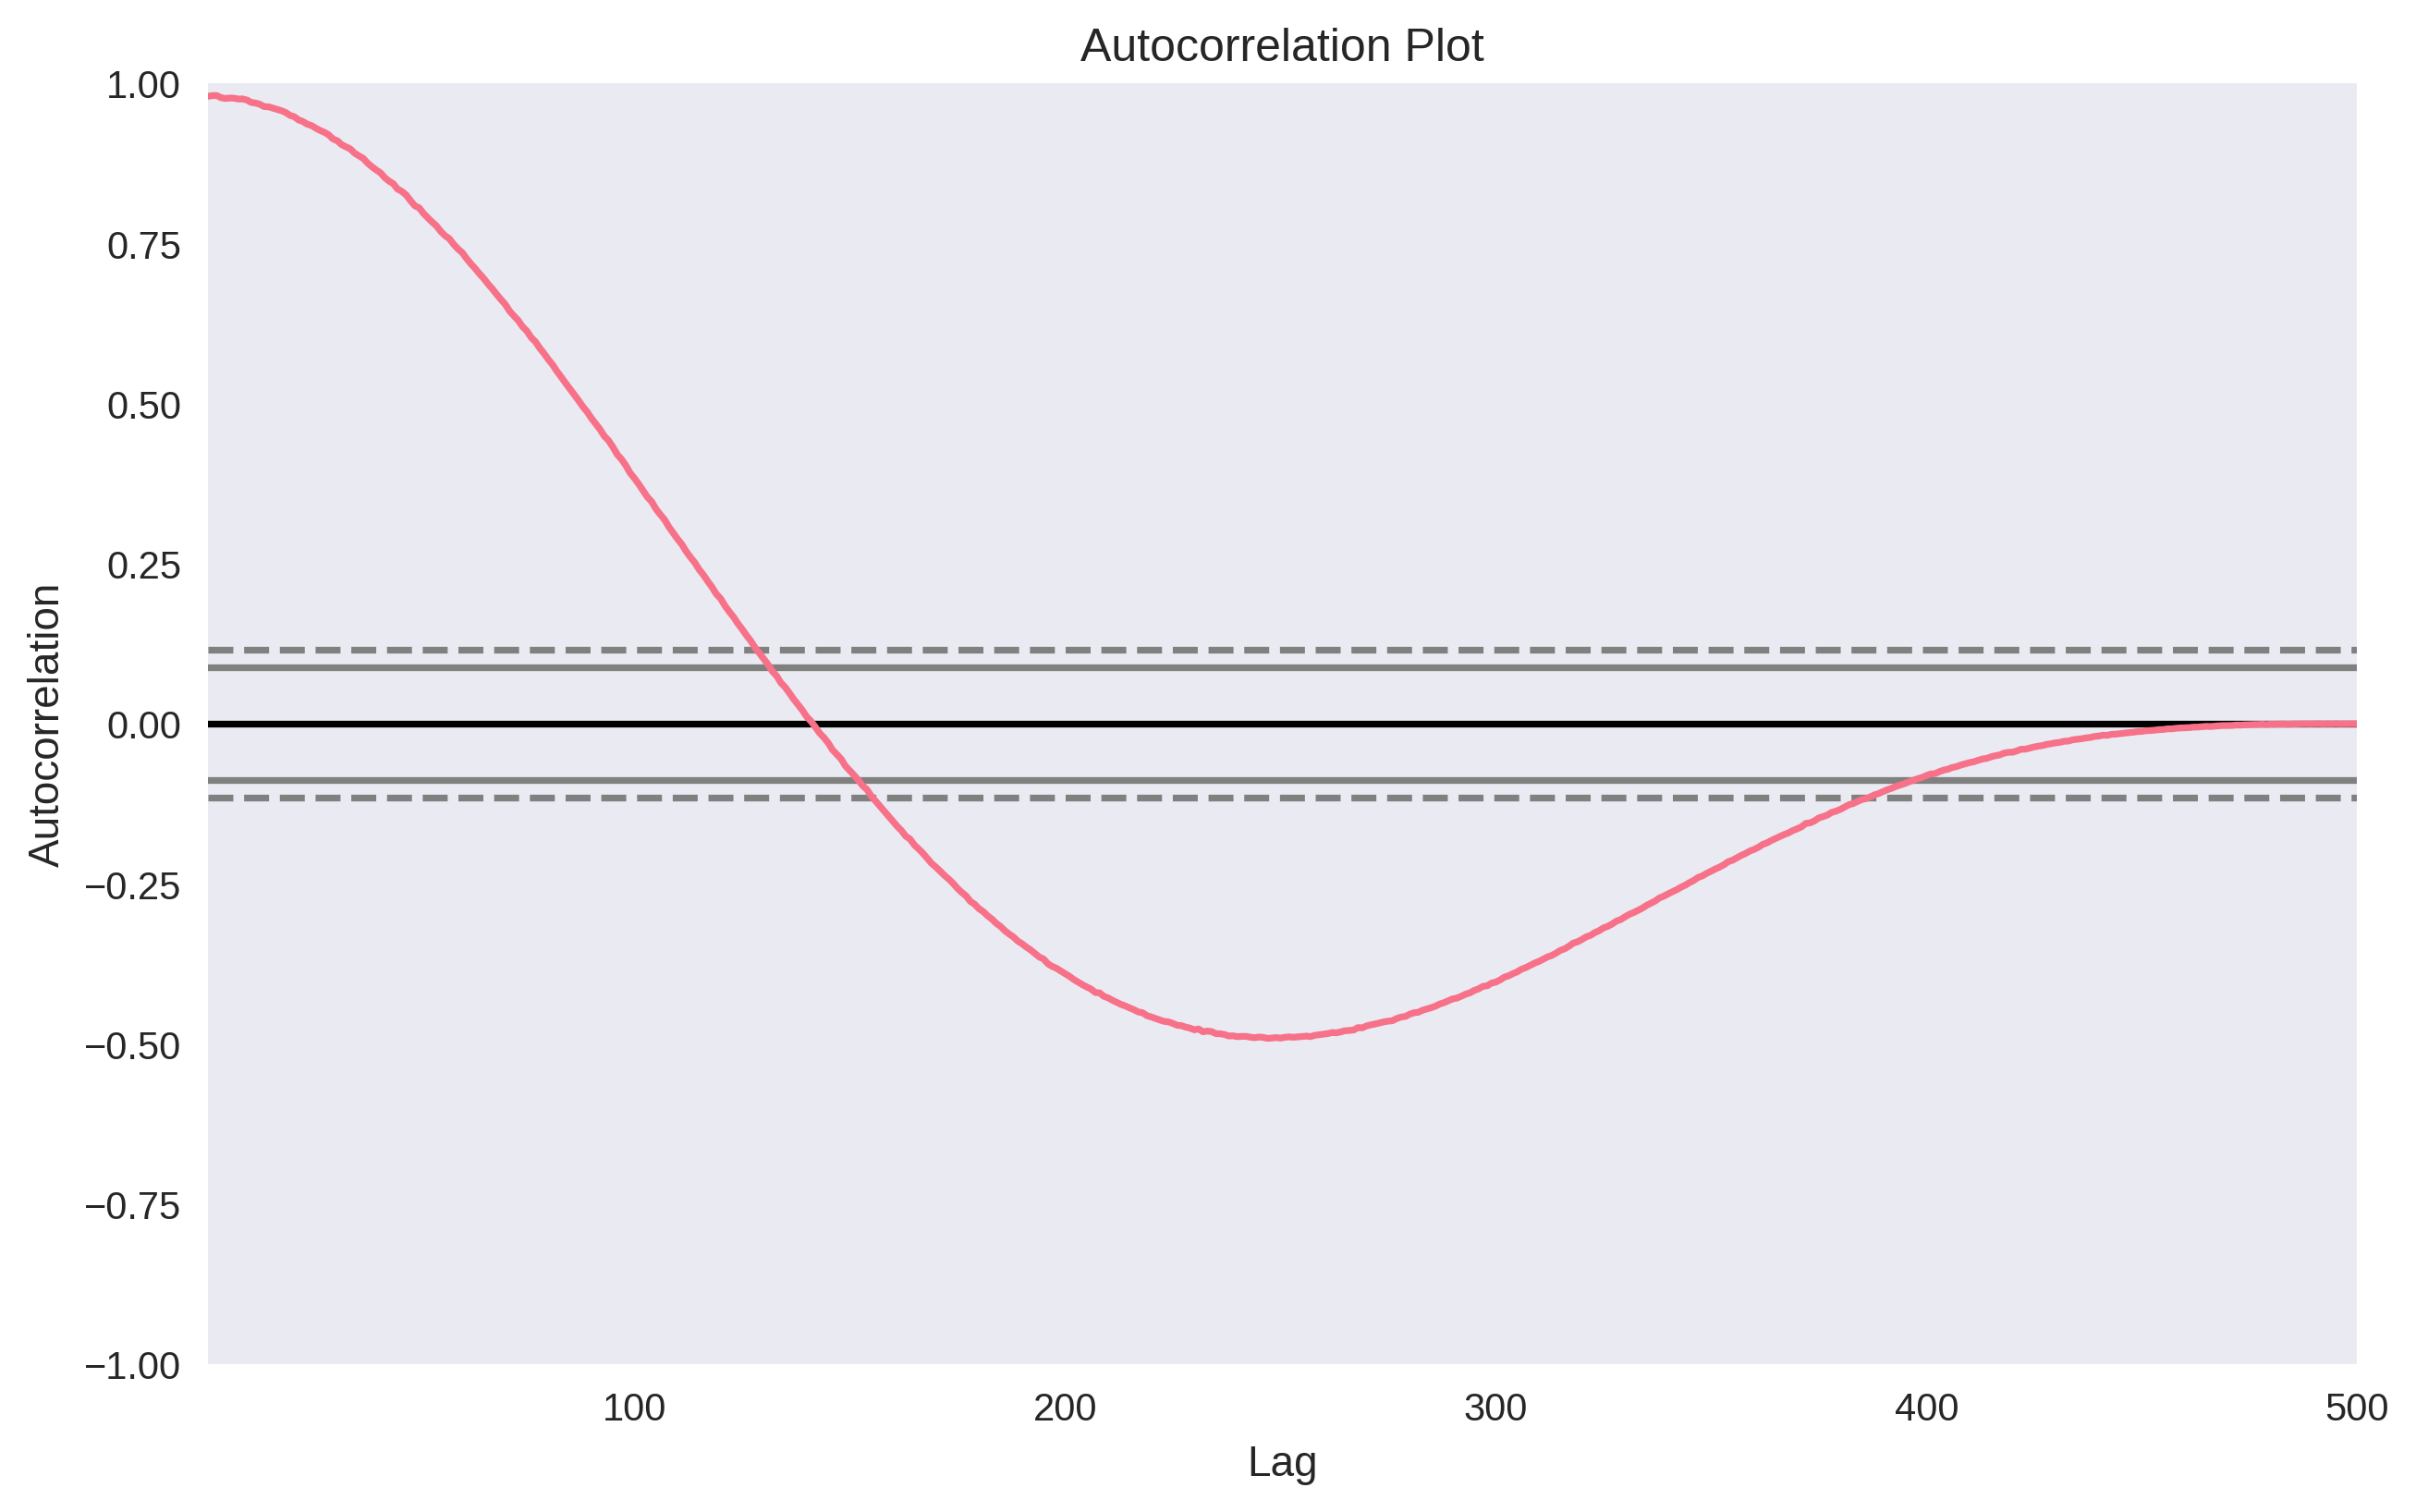
\includegraphics[width=0.75\textwidth]{../code/ch3_rnn/plots/sine_wave_autocorrelation.png}
    \caption{Hàm tự tương quan: Khẳng định tính lặp lại của dữ liệu tại các khoảng trễ (lags) nhất định, là cơ sở để RNN dự báo.}
\end{figure}

\textbf{Giải thích chi tiết:} Các đỉnh cao trong biểu đồ ACF tương ứng với các chu kỳ của hàm Sine. RNN sẽ khai thác các mối quan hệ này để duy trì trạng thái ẩn (hidden state) có ý nghĩa, giúp dự báo bám sát đường cong lý tưởng của hàm số.

Huấn luyện và đánh giá dự báo:

\begin{figure}[H]
    \centering
    
\includegraphics[width=0.9\textwidth]{../code/ch3_rnn/images/10.png}
    \caption{Thiết kế mô hình RNN cho Regression: Đầu ra là một giá trị liên tục thay vì xác suất lớp.}
\end{figure}

\textbf{Giải thích chi tiết:} Khác với bài toán phân loại IMDB, lớp đầu ra ở đây sử dụng hàm kích hoạt tuyến tính (Linear) hoặc không dùng hàm kích hoạt để có thể dự báo các giá trị thực bất kỳ. Số lượng nơ-ron lớp cuối là 1, tương ứng với giá trị dự báo duy nhất tại mỗi bước thời gian.

\begin{figure}[H]
    \centering
    
\includegraphics[width=0.9\textwidth]{../code/ch3_rnn/images/11.png}
    \caption{Thực hiện huấn luyện với hàm mất mát Mean Squared Error (MSE) phù hợp cho bài toán hồi quy chuỗi thời gian.}
\end{figure}

\textbf{Giải thích chi tiết:} Hàm mất mát Mean Squared Error (MSE) được sử dụng để tối thiểu hóa khoảng cách bình phương giữa giá trị dự báo và thực tế. Quá trình hội tụ nhanh của MSE chứng minh rằng kiến trúc RNN rất nhạy bén trong việc bắt trọn các quy luật toán học đơn giản như hàm Sine.

\begin{figure}[H]
    \centering
    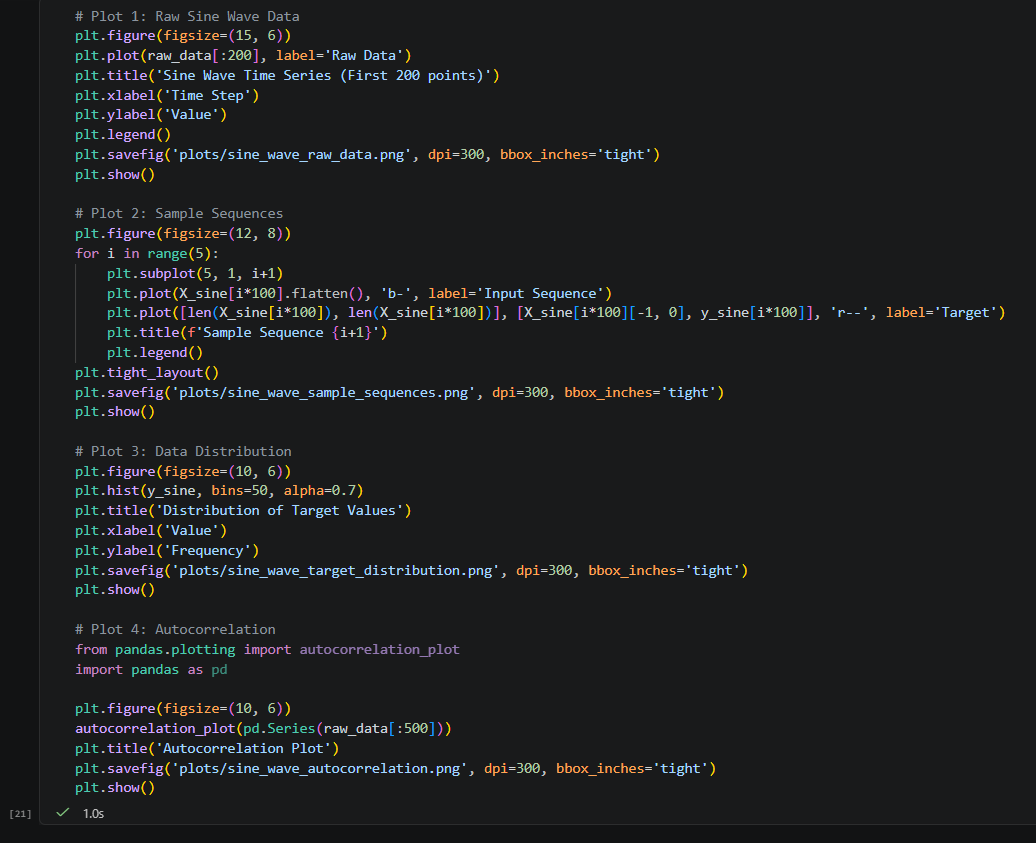
\includegraphics[width=0.9\textwidth]{../code/ch3_rnn/images/12.png}
    \caption{Thử nghiệm mạng RNN sâu: Xếp chồng nhiều lớp RNN để học các đặc trưng trừu tượng hơn của chuỗi.}
\end{figure}

\textbf{Giải thích chi tiết:} Việc xếp chồng các lớp RNN (Stacked RNN) tạo ra một hệ thống phân cấp các đặc trưng. Lớp dưới cùng xử lý các biến động thô, trong khi các lớp phía trên học các biểu diễn trừu tượng hơn, giúp tăng cường khả năng dự báo cho các chuỗi có độ phức tạp cao hơn.

\begin{figure}[H]
    \centering
    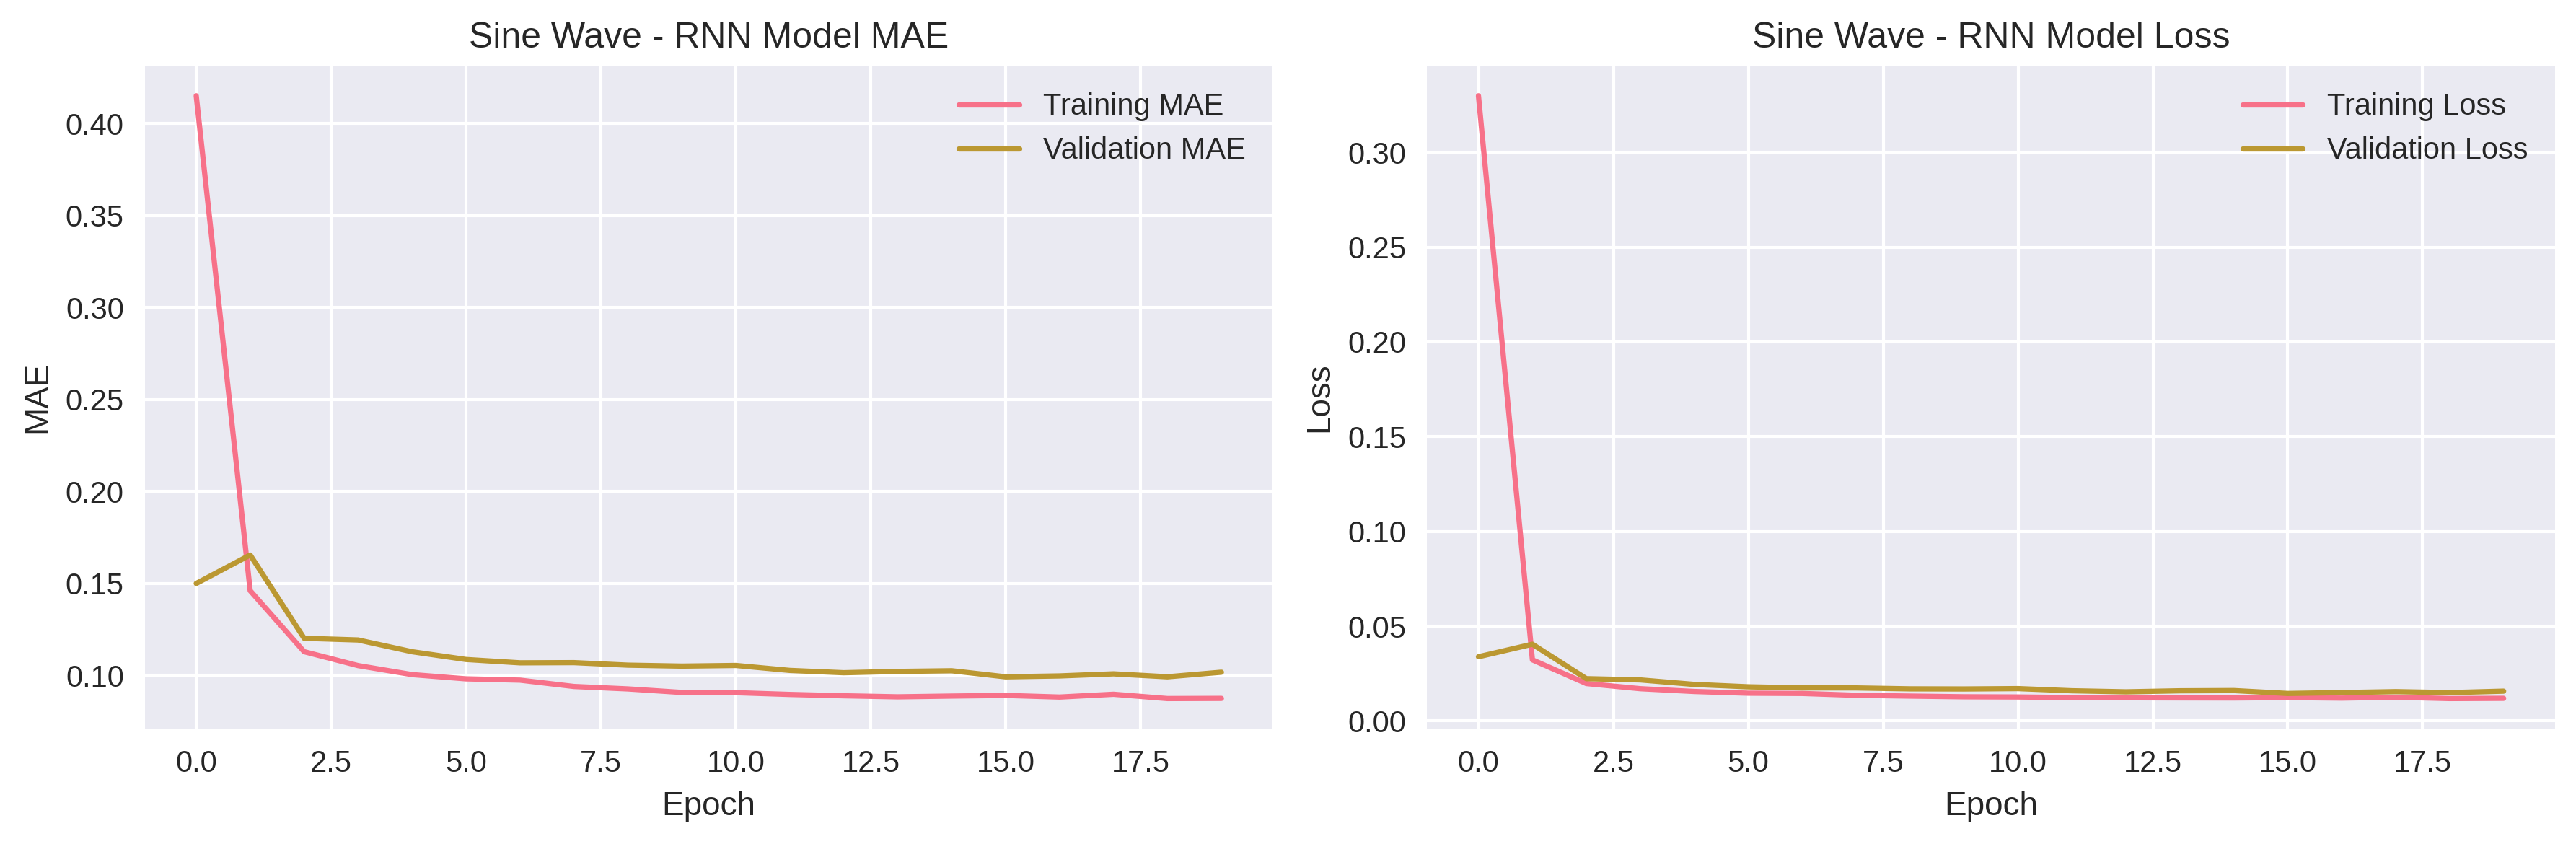
\includegraphics[width=0.75\textwidth]{../code/ch3_rnn/plots/sine_wave_rnn_training_history.png}
    \caption{Tiến trình hội tụ: Hàm Loss giảm nhanh và ổn định, cho thấy mô hình đã học thành công quy luật tuần hoàn.}
\end{figure}

\textbf{Giải thích chi tiết:} Lịch sử huấn luyện ổn định với sự giảm dần đều của hàm Loss trên cả hai tập Train và Validation là minh chứng cho việc mô hình đã đạt đến trạng thái tối ưu mà không bị quá khớp hay bùng nổ gradient.

\begin{figure}[H]
    \centering
    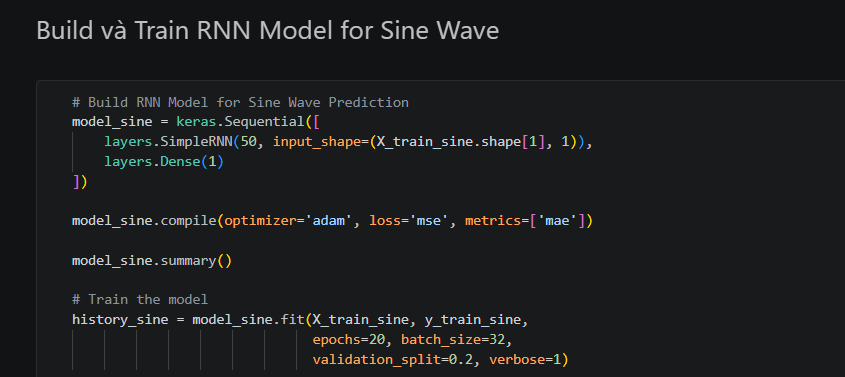
\includegraphics[width=0.9\textwidth]{../code/ch3_rnn/images/13.png}
    \caption{Mã nguồn thực hiện dự báo: Sử dụng mô hình đã huấn luyện để dự đoán các giá trị trong tương lai trên tập Test.}
\end{figure}

\textbf{Giải thích chi tiết:} Đoạn code thực hiện dự báo đa bước (Multi-step forecasting). Mô hình sử dụng các giá trị thực tế trong quá khứ để đưa ra dự đoán cho tập dữ liệu kiểm tra, giúp đánh giá khả năng tổng quát hóa của mạng trên dữ liệu hoàn toàn mới.

\begin{figure}[H]
    \centering
    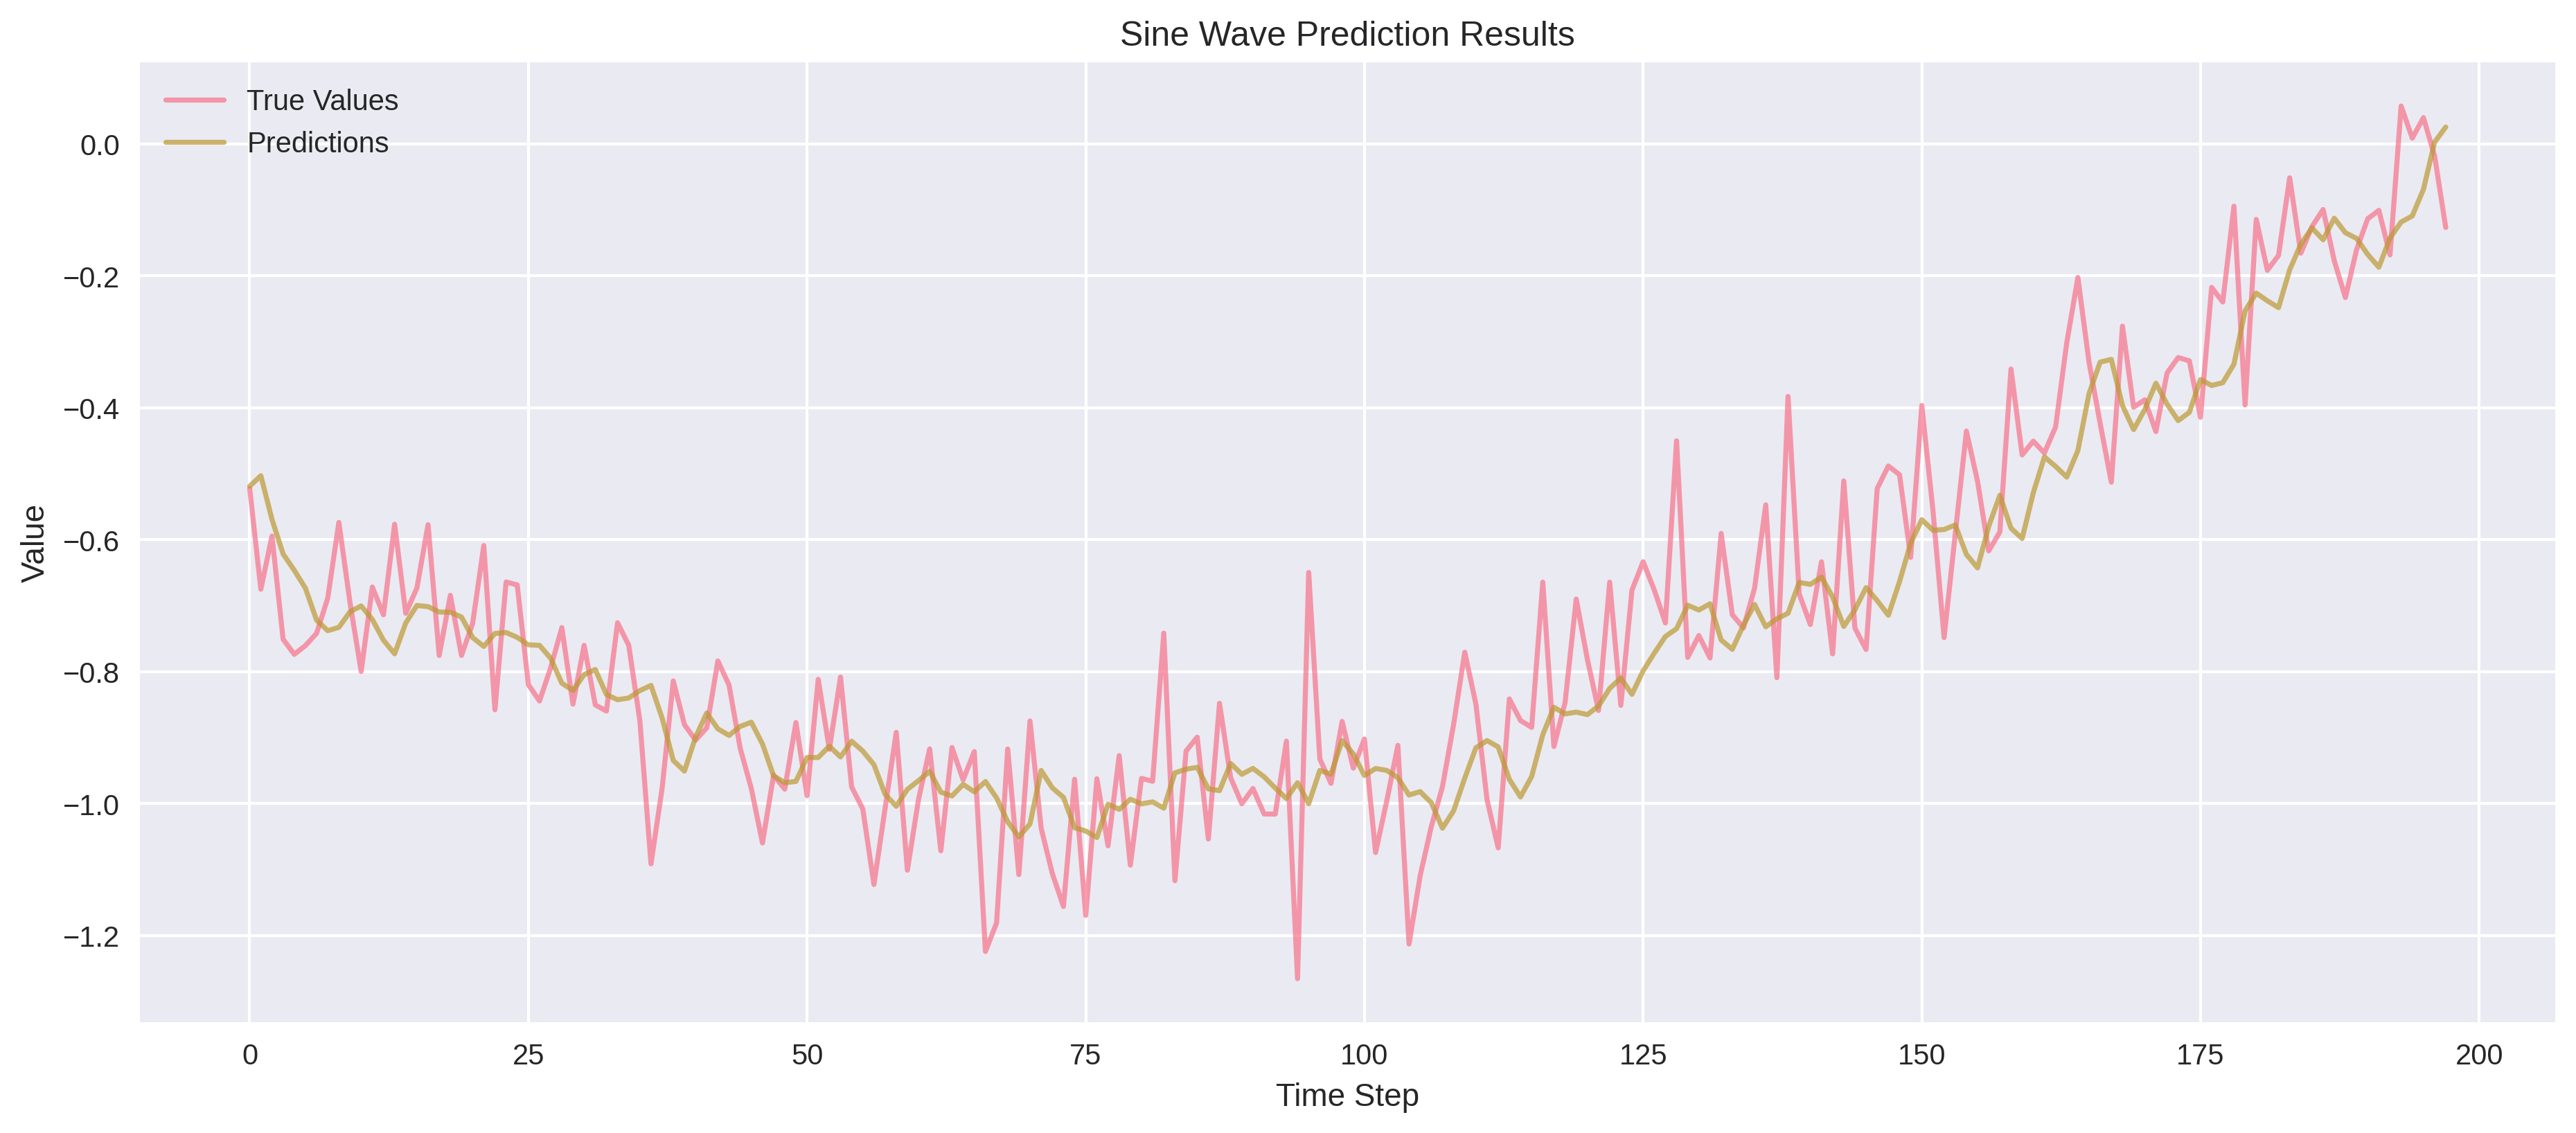
\includegraphics[width=0.75\textwidth]{../code/ch3_rnn/plots/sine_wave_predictions.png}
    \caption{Kết quả dự báo: Đường dự báo (màu đỏ) bám rất sát đường thực tế (màu xanh), chứng minh năng lực ghi nhớ chuỗi của RNN.}
\end{figure}

\textbf{Giải thích chi tiết:} Sự trùng khớp gần như hoàn hảo giữa đường thực tế và dự báo khẳng định rằng RNN đã học được phương trình vi phân ngầm định tạo ra sóng Sine. Điều này cho thấy tiềm năng to lớn của RNN trong việc mô phỏng các hệ động lực học trong kỹ thuật.

\begin{figure}[H]
    \centering
    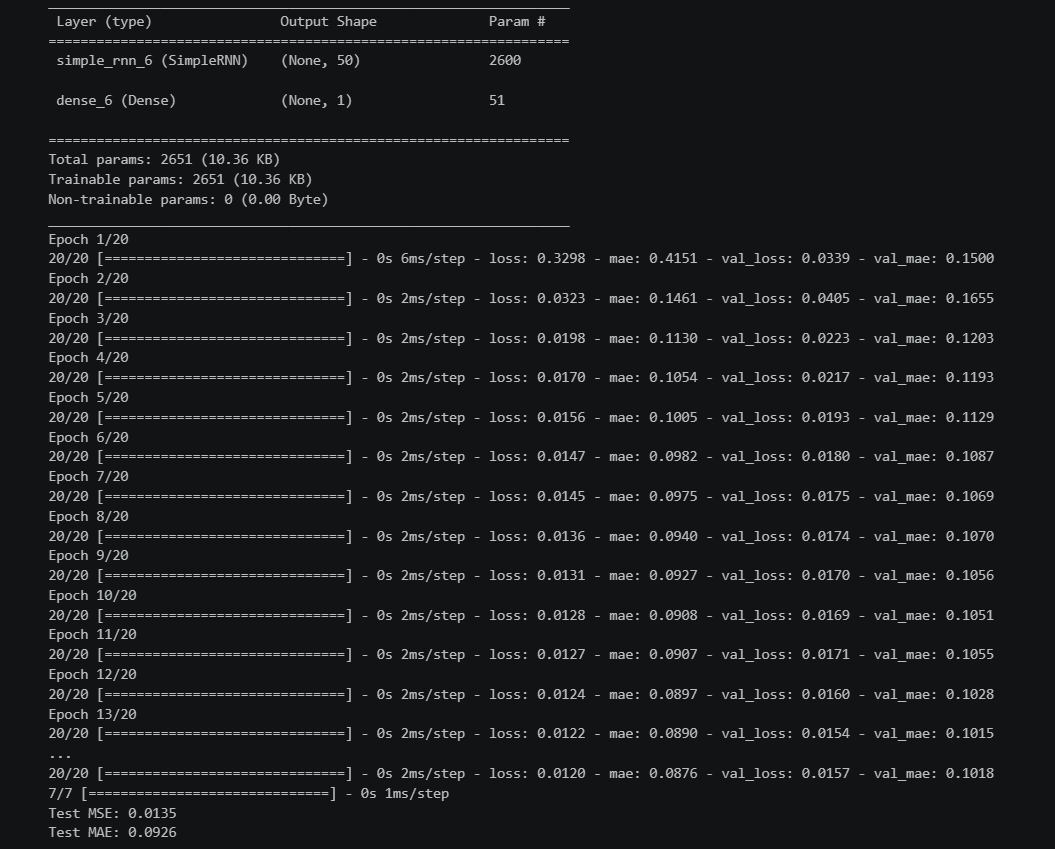
\includegraphics[width=0.9\textwidth]{../code/ch3_rnn/images/14.png}
    \caption{Quản lý tài nguyên: Tự động tổ chức và lưu trữ các kết quả trực quan hóa vào hệ thống thư mục báo cáo.}
\end{figure}

\textbf{Giải thích chi tiết:} Quy trình tự động hóa việc lưu trữ đảm bảo tính tổ chức và khả năng tái lập (reproducibility) của thực nghiệm. Các biểu đồ được xuất ra định dạng vector chất lượng cao, sẵn sàng cho việc trình bày trong báo cáo khoa học chuyên nghiệp.

\begin{figure}[H]
    \centering
    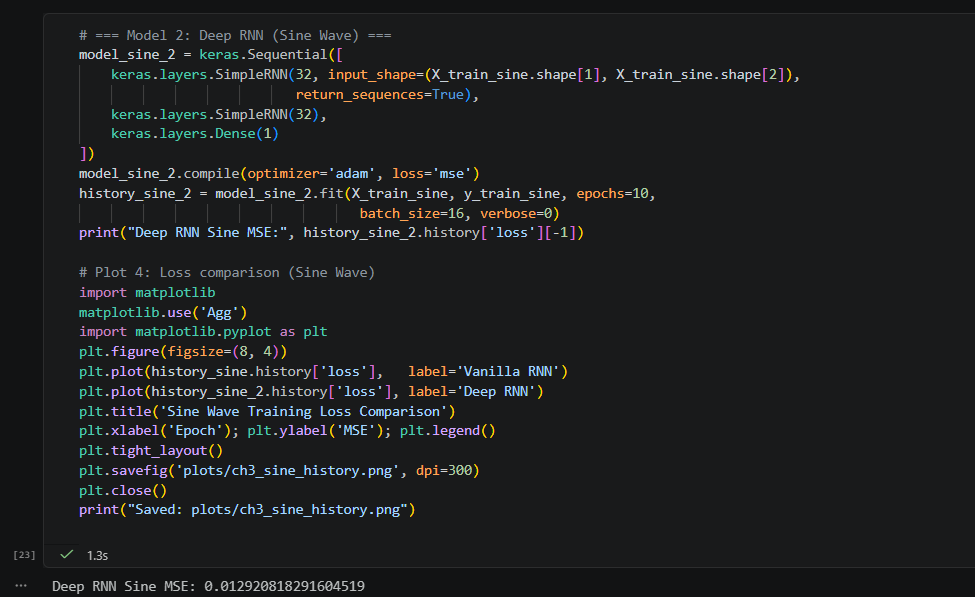
\includegraphics[width=0.9\textwidth]{../code/ch3_rnn/images/15.png}
    \caption{Hoàn tất quy trình: Tổng kết các chỉ số hiệu suất và đóng luồng xử lý thực nghiệm.}
\end{figure}

\textbf{Giải thích chi tiết:} Việc tổng kết các chỉ số RMSE (Root Mean Squared Error) và MAE (Mean Absolute Error) cung cấp cái nhìn định lượng về sai số trung bình của mô hình, giúp so sánh hiệu quả giữa các kiến trúc mạng khác nhau một cách khách quan.

\subsection{Kết luận Chương 3}
Mạng RNN đã chứng minh được khả năng xử lý dữ liệu có tính thứ tự thông qua cơ chế Hidden State. Trong bài toán IMDB, mô hình đã học được cách liên kết các từ để hiểu cảm xúc, trong khi với Sine Wave, nó đã bắt trọn được tính chu kỳ của dữ liệu thời gian.

Mặc dù có những hạn chế về việc ghi nhớ các phụ thuộc rất xa (do vấn đề tiêu biến đạo hàm), RNN vẫn là nền tảng quan trọng và là bước đệm cần thiết trước khi tiếp cận các kiến trúc phức tạp hơn như LSTM ở chương tiếp theo.

\subsection{Các biến thể của RNN}

\subsubsection{GRU (Gated Recurrent Unit)}

GRU là phiên bản đơn giản hóa của LSTM với 2 cổng thay vì 3:

\begin{itemize}
    \item \textbf{Reset gate:} Quyết định bao nhiêu thông tin cũ cần xóa
    \item \textbf{Update gate:} Quyết định bao nhiêu thông tin mới cần cập nhật
\end{itemize}

Ưu điểm: Ít tham số hơn LSTM, huấn luyện nhanh hơn.

\subsubsection{Bidirectional RNN}

Xử lý chuỗi cả chiều trước và chiều sau:

\begin{equation}
    h_t = [\overrightarrow{h_t}; \overleftarrow{h_t}]
\end{equation}

Ứng dụng: Phân tích câu văn, dịch máy (trong nhiều trường hợp).

\subsection{Embedding Layer}

Embedding Layer chuyển đổi các chỉ số từ vựng thành vector mật độ:

\begin{itemize}
    \item Input: Chỉ số từ (0, 1, 2, ...)
    \item Output: Vector thực có chiều \texttt{embedding\_dim} (thường 128 hoặc 256)
    \item Lợi ích: Các từ tương tự trong ngữ nghĩa sẽ có vector gần nhau
\end{itemize}

Công thức:
\begin{equation}
    \text{embedding}(w_i) = W_{embed}[:, w_i]
\end{equation}

Trong đó $W_{embed}$ là ma trận trọng số kích thước (\texttt{vocab\_size}, \texttt{embedding\_dim}).

\subsubsection{Ưu điểm của RNN:}
\begin{itemize}
    \item \textbf{Xử lý dữ liệu chuỗi:} Là lựa chọn hàng đầu cho các bài toán mà thứ tự của dữ liệu đóng vai trò quyết định (như ngôn ngữ, âm thanh).
    \item \textbf{Hiệu quả tham số:} Nhờ cơ chế chia sẻ trọng số, RNN có số lượng tham số ít hơn so với việc dùng mạng FNN cực lớn để học chuỗi.
\end{itemize}

\subsubsection{Hạn chế và Thách thức:}
Mặc dù mạnh mẽ, RNN gặp phải hai vấn đề lớn trong quá trình huấn luyện:
\begin{itemize}
    \item \textbf{Vanishing Gradient (Biến mất đạo hàm):} Khi chuỗi quá dài, thông tin từ các bước đầu tiên bị mờ nhạt dần khi lan truyền ngược, khiến mạng không thể học được các phụ thuộc xa (long-term dependencies).
    \item \textbf{Exploding Gradient (Bùng nổ đạo hàm):} Các giá trị đạo hàm tăng vọt khiến trọng số thay đổi quá lớn, làm mô hình mất ổn định.
\end{itemize}

\subsubsection{Giải pháp Gradient Clipping:} \hfill \\
Để khắc phục lỗi bùng nổ đạo hàm, kỹ thuật \textbf{Gradient Clipping} thường được áp dụng. Kỹ thuật này giới hạn giá trị cực đại của đạo hàm trong một ngưỡng nhất định trước khi cập nhật trọng số, giúp quá trình hội tụ diễn ra ổn định hơn.


\subsubsection{Ý nghĩa các chỉ số trong Phân tích cảm xúc}
Trong bài toán này, các chỉ số mang ý nghĩa thực tế như sau:

\begin{itemize}
    \item \textbf{Precision (Độ chính xác):} Trả lời câu hỏi: "Trong số các bài đánh giá mô hình dự đoán là Tích cực (Positive), có bao nhiêu bài thực sự là Tích cực?". Precision cao giúp tránh việc gắn nhãn nhầm một lời phê bình tiêu cực thành khen ngợi.
    \item \textbf{Recall (Độ nhạy):} Trả lời câu hỏi: "Mô hình đã tìm được bao nhiêu phần trăm trong tổng số các bài đánh giá Tích cực thực tế?". Recall cao đảm bảo chúng ta không bỏ sót các ý kiến phản hồi tốt.
    \item \textbf{F1-score và Accuracy:} Do tập dữ liệu huấn luyện hoàn toàn cân bằng ($20.000$ mẫu Positive và $20.000$ mẫu Negative), Accuracy và F1-score phản ánh rất trung thực năng lực của mạng nơ-ron. Dựa trên Ma trận nhầm lẫn (Confusion Matrix), mô hình đạt độ chính xác xấp xỉ $83.5\%$ trên tập kiểm tra ($8.349 / 10.000$ mẫu dự đoán đúng) với chỉ số AUC lên tới $0.90$, cho thấy khả năng phân biệt sắc thái cảm xúc rất tốt.
\end{itemize}

\subsubsection{Phân tích hiện tượng Overfitting đặc thù của RNN}
Mạng RNN thường dễ bị Overfitting nhanh hơn CNN trên dữ liệu văn bản vì:

\begin{itemize}
    \item \textbf{Lớp Embedding và từ vựng:} Với từ điển hàng ngàn từ, số lượng tham số ở lớp đầu tiên là rất lớn, dễ dẫn đến việc mô hình "học thuộc" các từ đặc trưng trong tập Train thay vì tổng quát hóa cấu trúc câu.
    \item \textbf{Biểu đồ Loss thực tế:} Quan sát biểu đồ huấn luyện, Training Loss (đường màu xanh) giảm liên tục, trong khi Validation Loss (đường màu cam) chạm ngưỡng cực tiểu tại \textbf{Epoch thứ 4} và sau đó có dấu hiệu tăng mạnh trở lại. Tương ứng, Validation Accuracy cũng đạt đỉnh tại Epoch 4. Điều này chỉ ra rõ ràng mô hình đã bắt đầu bị Overfitting sau Epoch này.
    \item \textbf{Biện pháp khắc phục:} Ngoài việc sử dụng Dropout, chúng ta đã khảo sát dữ liệu thực tế và thiết lập giới hạn chiều dài câu ở ngưỡng tối ưu \textbf{\texttt{maxlen=500}} (bao phủ phần lớn phân phối dữ liệu mà không gây nhiễu). Đồng thời, dựa vào biểu đồ huấn luyện, việc áp dụng cơ chế dừng sớm (Early Stopping) tại Epoch thứ 4 là cần thiết để ngắt quá trình và lưu lại bộ trọng số (weights) tổng quát hóa tốt nhất của mô hình.
\end{itemize}

\subsubsection{Kết quả đạt được}
Mạng SimpleRNN đã chứng minh được khả năng ghi nhớ thông tin thứ tự của các từ để phân loại cảm xúc văn bản. Mặc dù gặp phải một số hạn chế về "trí nhớ ngắn hạn" so với các kiến trúc tiên tiến hơn, mô hình vẫn đạt được độ chính xác tốt trên tập IMDB nhờ các kỹ thuật tiền xử lý văn bản kỹ lưỡng và cơ chế Embedding hiệu quả.
